\documentclass[12pt]{article}
\usepackage{amsmath, amssymb, amsthm}
\usepackage{mathtools}
\usepackage{graphicx}
\usepackage{float}
\usepackage{hyperref}
\usepackage{xcolor}
\usepackage{listings}
\usepackage{geometry}
\usepackage{algorithm}
\usepackage{algpseudocode}
\usepackage{tikz}
\usepackage{longtable}
\usepackage{circuitikz}
\usepackage{comment}
\usepackage{MnSymbol}
\usepackage{physics}
\usepackage[section]{placeins}

\title{Bandpass Filter using Sallen-Key Second-Order Filters}
\author{Abhimanyu Koushik (EE24BTECH11024),\\Agamjot Singh (EE24BTECH11002)\\IIT Hyderabad}
\date{\today}

\begin{document}

\maketitle

\section{Introduction}

Bandpass filters are essential components in signal processing systems, allowing frequencies within a specific range to pass while attenuating frequencies outside this range. This experiment focuses on implementing a bandpass filter using the Sallen-Key topology, which is widely used for its simplicity and stability. The bandpass filter is constructed by cascading a high-pass filter (HPF) and a low-pass filter (LPF), with carefully selected cutoff frequencies to define the desired passband.

\section{Theory}

\subsection{Bandpass Filter Fundamentals}

A bandpass filter (BPF) allows signals within a specific frequency range to pass while attenuating signals outside this range. The filter is characterized by:
\begin{itemize}
    \item Lower cutoff frequency ($f_{l}$): Frequencies below this are attenuated
    \item Upper cutoff frequency ($f_{h}$): Frequencies above this are attenuated
    \item Bandwidth $ = f_{h} - f_{l}$
    \item Center frequency ($f_0$) $ = \sqrt{f_{h} \times f_{l}}$
\end{itemize}

\newpage
\subsection{High Pass Filter Topology}

\begin{figure}[!htbp]
\centering
\resizebox{0.49\textwidth}{!}{%
\begin{circuitikz}
\tikzstyle{every node}=[font=\LARGE]
\draw (3.75,12.5) to[short] (6,12.5);
\draw (8,12.5) to[short] (8,14.25);
\draw (8,14.25) to[short] (10.75,14.25);
\draw (12.75,12.5) node[op amp,scale=1, yscale=-1 ] (opamp2) {};
\draw (opamp2.+) to[short] (11.25,13);
\draw  (opamp2.-) to[short] (11.25,12);
\draw (13.95,12.5) to[short](14.25,12.5);
\draw (13,14.25) to[short] (14.25,14.25);
\draw (14.25,14.25) to[short] (14.25,12.5);
\draw (10,12.5) to[short] (10,13);
\draw (10,13) to[short] (11.5,13);
\draw (11.25,12) to[short] (11.25,10.75);
\draw (11.25,10.75) to[short] (14.25,10.75);
\draw (14.25,10.5) to[short] (14.25,13);
\draw (14.25,10.75) to[R] (14.25,8.75);
\draw (10,10.25) to (10,10) node[ground]{};
\draw (14.25,8.75) to (14.25,8.25) node[ground]{};
\node [font=\large] at (3.5,12.5) {$V_{in}$};
\node [font=\large] at (14.75,12.5) {$V_{out}$};
\node [font=\large] at (9.5,11.25) {$R_1$};
\node [font=\large] at (11.75,15) {$R_2$};
\node [font=\large] at (9,11.75) {$C_2$};
\node [font=\large] at (7,11.75) {$C_1$};
\node [font=\large] at (15,9.75) {$R_f$};
\draw (6,12.5) to[C] (8,12.5);
\draw (8,12.5) to[C] (10,12.5);
\draw (10,12.5) to[R] (10,10.25);
\draw (10.5,14.25) to[R] (13,14.25);
\end{circuitikz}
}%
\end{figure}
\FloatBarrier
Given the circuit diagram, we write the equations as follows:

\begin{equation*}
\frac{V_{\text{in}} - V_1}{X_{C_1}} + \frac{V_2 - V_1}{X_{C_2}} + \frac{V_{\text{out}} - V_1}{R_2} = 0
\end{equation*}

Simplifying:

\begin{equation*}
\frac{V_{\text{in}}}{X_{C_1}} + \frac{V_2}{X_{C_2}} + \frac{V_{\text{out}}}{R_2} = V_1 \left( \frac{1}{X_{C_1}} + \frac{1}{X_{C_2}} + \frac{1}{R_2} \right)
\end{equation*}

Next, consider the relationship between $V_1$ and $V_2$:

\begin{equation*}
\frac{V_1 - V_2}{X_{C_2}} - \frac{V_2}{R_1} = 0
\end{equation*}

Rewriting:

\begin{equation*}
V_1 = V_2 \left( 1 + \frac{X_{C_2}}{R_1} \right)
\end{equation*}

Using the virtual short property ($V_2 = V_{\text{out}}$):

\begin{equation*}
V_1 = V_{\text{out}} \left( 1 + \frac{X_{C_2}}{R_1} \right)
\end{equation*}

Substituting $X_{C_1}$ and $X_{C_2}$ as:

\begin{equation*}
X_{C_1} = \frac{1}{j\omega C_1}, \quad X_{C_2} = \frac{1}{j\omega C_2}
\end{equation*}

We get:

\begin{equation*}
V_1 = V_{\text{out}} \left( 1 + \frac{1}{j\omega C_1 R_2} \right)
\end{equation*}

Substituting back into the first equation:

\begin{equation*}
\frac{V_{\text{in}}}{X_{C_1}} + \frac{V_{\text{out}}}{R_2} + j\omega C_2V_{\text{out}} = V_{\text{out}} \left( 1 + \frac{1}{j\omega C_1 R_2} \right) \left( \frac{1}{R_2} + j\omega C_1 + j\omega C_2 \right)
\end{equation*}

Expanding further:

\begin{equation*}
\frac{V_{\text{in}}}{X_{C_1}} + V_{\text{out}} \left( \frac{1}{R_2} + j\omega C_2 \right) = V_{\text{out}} \left( 1 + \frac{1}{j\omega C_1 R_2} \right) \left( \frac{1}{R_2} + j\omega C_1 + j\omega C_2 \right)
\end{equation*}

Rewriting the transfer function:

\begin{equation*}
s^2 V_{\text{in}} C_1 C_2 R_1 R_2= V_{\text{out}} \left( 1 + s R_2 (C_1 + C_2) + s^2 C_1 C_2 R_1 R_2 \right)
\end{equation*}

\begin{equation*}
H(s) = \frac{V_{\text{out}}}{V_{\text{in}}} = \frac{s^2C_1 C_2 R_1 R_2}{s^2 C_1 C_2 R_1 R_2 + s R_2 (C_1 + C_2) + 1}
\end{equation*}

Assume $C_1 = C_2 = C$ and $R_1 = R_2 = R$,
\begin{align*}
    \text{Gain} = \abs{H(s)} = \frac{(\omega RC)^2}{(\omega RC)^2 + 1}
\end{align*}

Cutoff angular frequency ($w_c$) is given by,
\begin{align*}
    w_c = \frac{1}{RC}
\end{align*}

Cutoff frequency ($f_c$) is given by,
\begin{align*}
    f_c = \frac{1}{2\pi RC}
\end{align*}

\newpage
\subsection{Low-Pass Filter Topology}

\begin{figure}[!ht]
\centering
\resizebox{0.5\textwidth}{!}{%
\begin{circuitikz}
\tikzstyle{every node}=[font=\large]
\draw (3.75,12.5) to[short] (6,12.5);
\draw (6,12.5) to[R] (7.75,12.5);
\draw (7.75,12.5) to[R] (10,12.5);
\draw (10,12.5) to[C] (10,10);
\draw (8,12.5) to[short] (8,14.25);
\draw (8,14.25) to[short] (10.75,14.25);
\draw (12.75,12.5) node[op amp,scale=1, yscale=-1 ] (opamp2) {};
\draw (opamp2.+) to[short] (11.25,13);
\draw  (opamp2.-) to[short] (11.25,12);
\draw (13.95,12.5) to[short](14.25,12.5);
\draw (10.75,14.25) to[C] (13.25,14.25);
\draw (13,14.25) to[short] (14.25,14.25);
\draw (14.25,14.25) to[short] (14.25,12.5);
\draw (10,12.5) to[short] (10,13);
\draw (10,13) to[short] (11.5,13);
\draw (11.25,12) to[short] (11.25,10.75);
\draw (11.25,10.75) to[short] (14.25,10.75);
\draw (14.25,10.5) to[short] (14.25,13);
\draw (14.25,10.75) to[R] (14.25,8.75);
\draw (10,10.25) to (10,10) node[ground]{};
\draw (14.25,8.75) to (14.25,8.25) node[ground]{};
\node [font=\large] at (3.5,12.5) {$V_{in}$};
\node [font=\large] at (14.75,12.5) {$V_{out}$};
\node [font=\large] at (7,12) {$R_1$};
\node [font=\large] at (9,12) {$R_2$};
\node [font=\large] at (12,15) {$C_2$};
\node [font=\large] at (9.25,10.75) {$C_1$};
\node [font=\large] at (15,9.75) {$R_f$};
\end{circuitikz}
}%
\end{figure}
\FloatBarrier

Given the circuit diagram, we write the equations as follows:

\begin{equation}
\frac{V_{\text{in}} - V_1}{R_1} + \frac{V_2 - V_1}{R_2} + \frac{V_{\text{out}} - V_1}{X_{C_2}} = 0
\end{equation}

Simplifying:

\begin{equation}
\frac{V_{\text{in}}}{R_1} + \frac{V_2}{R_2} + \frac{V_{\text{out}}}{X_{C_2}} = V_1 \left( \frac{1}{R_1} + \frac{1}{R_2} + \frac{1}{X_{C_2}} \right)
\end{equation}

Next, consider the relationship between $V_1$ and $V_2$:

\begin{equation}
\frac{V_1 - V_2}{R_2} - \frac{V_2}{X_{C_1}} = 0
\end{equation}

Rewriting:

\begin{equation}
V_1 = V_2 \left( 1 + \frac{R_2}{X_{C_1}} \right)
\end{equation}

Using the virtual short property ($V_2 = V_{\text{out}}$):

\begin{equation}
V_1 = V_{\text{out}} \left( 1 + \frac{R_2}{X_{C_1}} \right)
\end{equation}

Substituting $X_{C_1}$ and $X_{C_2}$ as:

\begin{equation}
X_{C_1} = \frac{1}{j\omega C_1}, \quad X_{C_2} = \frac{1}{j\omega C_2}
\end{equation}

We get:

\begin{equation}
V_1 = V_{\text{out}} \left( 1 + j\omega C_1 R_2 \right)
\end{equation}

Substituting back into the first equation:

\begin{equation}
\frac{V_{\text{in}}}{R_1} + \frac{V_{\text{out}}}{R_2} + j\omega C_2 V_{\text{out}}= V_{\text{out}} ( 1 + j\omega C_1 R_2 ) \left( \frac{1}{R_1} + \frac{1}{R_2} + j\omega C_2 \right)
\end{equation}

Expanding further:

\begin{equation}
\frac{V_{\text{in}}}{R_1} + V_{\text{out}} \left( \frac{1}{R_2} + j\omega C_2 \right) = V_{\text{out}} \left( 1 + j\omega C_1 R_2 \right) \left( \frac{1}{R_1} + \frac{1}{R_2} + j\omega C_2 \right)
\end{equation}

Rewriting the transfer function:

\begin{equation}
V_{\text{in}} = V_{\text{out}} \left( 1 + s C_1 (R_1 + R_2) + s^2 C_1 C_2 R_1 R_2 \right)
\end{equation}

\begin{equation}
H(s) = \frac{V_{\text{out}}}{V_{\text{in}}} = \frac{1}{s^2 C_1 C_2 R_1 R_2 + s C_1 (R_1 + R_2) + 1}
\end{equation}


Assume $C_1 = C_2 = C$ and $R_1 = R_2 = R$,
\begin{align*}
     \text{Gain} = \abs{H(s)} = \frac{1}{(\omega RC)^2 + 1}
\end{align*}

Cutoff angular frequency ($w_c$) is given by,
\begin{align*}
    w_c = \frac{1}{RC}
\end{align*}

Cutoff frequency ($f_c$) is given by,
\begin{align*}
    f_c = \frac{1}{2\pi RC}
\end{align*}

\subsection{Band-Pass Filter Topology}
Band-Pass Filter is just low-pass and high-pass filters cascaded, i.e. output of low-pass filter is passed to high-pass filter and the final out is $V_{out}$ of high-pass filter.

\begin{figure}[!ht]
\centering
\resizebox{1\textwidth}{!}{%
\begin{circuitikz}
\tikzstyle{every node}=[font=\large]
\draw (3.75,12.5) to[short] (6,12.5);
\draw (8,12.5) to[short] (8,14.25);
\draw (8,14.25) to[short] (10.75,14.25);
\draw (12.75,12.5) node[op amp,scale=1, yscale=-1 ] (opamp2) {};
\draw (opamp2.+) to[short] (11.25,13);
\draw  (opamp2.-) to[short] (11.25,12);
\draw (13.95,12.5) to[short](14.25,12.5);
\draw (13,14.25) to[short] (14.25,14.25);
\draw (14.25,14.25) to[short] (14.25,12.5);
\draw (10,12.5) to[short] (10,13);
\draw (10,13) to[short] (11.5,13);
\draw (11.25,12) to[short] (11.25,10.75);
\draw (11.25,10.75) to[short] (14.25,10.75);
\draw (14.25,10.5) to[short] (14.25,13);
\draw (14.25,10.75) to[R] (14.25,8.75);
\draw (10,10.25) to (10,10) node[ground]{};
\draw (14.25,8.75) to (14.25,8.25) node[ground]{};
\node [font=\large] at (3.5,12.5) {$V_{in}$};
\node [font=\large] at (7,12) {$R_1$};
\node [font=\large] at (9,12) {$R_1$};
\node [font=\large] at (11.75,15) {$C_1$};
\node [font=\large] at (9.25,11.25) {$C_1$};
\node [font=\large] at (15,9.75) {$R_f$};
\draw (13.75,12.5) to[short] (16,12.5);
\draw (18,12.5) to[short] (18,14.25);
\draw (18,14.25) to[short] (20.75,14.25);
\draw (22.75,12.5) node[op amp,scale=1, yscale=-1 ] (opamp2) {};
\draw (opamp2.+) to[short] (21.25,13);
\draw  (opamp2.-) to[short] (21.25,12);
\draw (23.95,12.5) to[short](24.25,12.5);
\draw (23,14.25) to[short] (24.25,14.25);
\draw (24.25,14.25) to[short] (24.25,12.5);
\draw (20,12.5) to[short] (20,13);
\draw (20,13) to[short] (21.5,13);
\draw (21.25,12) to[short] (21.25,10.75);
\draw (21.25,10.75) to[short] (24.25,10.75);
\draw (24.25,10.5) to[short] (24.25,13);
\draw (24.25,10.75) to[R] (24.25,8.75);
\draw (20,10.25) to (20,10) node[ground]{};
\draw (24.25,8.75) to (24.25,8.25) node[ground]{};
\node [font=\large] at (24.75,12.5) {$V_{out}$};
\node [font=\large] at (19.5,11.25) {$R_2$};
\node [font=\large] at (21.75,15) {$R_2$};
\node [font=\large] at (19,11.75) {$C_2$};
\node [font=\large] at (17,11.75) {$C_2$};
\node [font=\large] at (25,9.75) {$R_f$};
\draw (16,12.5) to[C] (18,12.5);
\draw (18,12.5) to[C] (20,12.5);
\draw (20,12.5) to[R] (20,10.25);
\draw (20.5,14.25) to[R] (23,14.25);
\draw (6,12.5) to[R] (8,12.5);
\draw (8,12.5) to[R] (10,12.5);
\draw (10.5,14.25) to[C] (13,14.25);
\draw (10,12.5) to[C] (10,10.25);
\end{circuitikz}
}%
\end{figure}
\FloatBarrier

Cutoff frequency (low-pass): $ f_{low}= \frac{1}{R_1 C_1}$.\newline

Cutoff frequency (high-pass): $ f_{high} = \frac{1}{R_2 C_2}$.\newline

Bandwidth $= f_{low} - f_{high} = \frac{1}{R_1 C_1} - \frac{1}{R_2 C_2}$.

\section{Apparatus}
\begin{itemize}
    \item Operational Amplifiers
    \item Resistors: $R_1, R_2, R_3, R_4$ (in k$\Omega$)
    \item Capacitors: $C_1, C_2, C_3, C_4$ (in nF)
    \item Function Generator
    \item Oscilloscope
    \item DC Power Supply
    \item Breadboard and connecting wires
\end{itemize}

\section{Procedure}
\subsubsection{High-Pass Filter Implementation}
\begin{enumerate}
    \item Assemble the Sallen-Key HPF circuit on the breadboard.
    \item Connect the function generator to the input and set it to generate a sine wave.
    \item Connect the oscilloscope to measure the output voltage.
    \item Vary the input frequency from 100 Hz to 100 kHz in appropriate steps.
    \item For each frequency, record the input and output voltages to calculate the gain.
    \item Plot the frequency response (gain vs. frequency) on a logarithmic scale.
\end{enumerate}

\subsubsection{Low-Pass Filter Implementation}
\begin{enumerate}
    \item Assemble the Sallen-Key LPF circuit on the breadboard.
    \item Repeat the same procedure as in Step 1.
\end{enumerate}

\subsubsection{Bandpass Filter Implementation}
\begin{enumerate}
    \item Connect the output of the LPF to the input of the HPF to form the complete bandpass filter.
    \item Repeat the frequency response measurements as in the previous steps.
\end{enumerate}

\newpage
\section{Results and Analysis}
\subsection{Low-Pass Filter}

\begin{align*}
    R = 1k\Omega, C = 85nF
\end{align*}

\begin{table}[h]
\centering
\begin{tabular}{|c|c|}
\hline
$\log(\omega)$ & $20 \log(|H(s)|)$ \\
\hline
1.7982 & -0.7242 \\
2.4971 & 0.0 \\
2.7982 & 0.0 \\
3.0992 & 0.0 \\
3.4971 & -0.3546 \\
3.7013 & -1.1103 \\
3.7982 & -1.9382 \\
3.8774 & -2.2905 \\
3.9743 & -3.6593 \\
4.0992 & -5.8112 \\
4.2753 & -10.5683 \\
4.4002 & -14.3340 \\
4.4971 & -16.8328 \\
4.5763 & -19.0156 \\
4.6732 & -21.9382 \\
4.7982 & -25.0362 \\
\hline
\end{tabular}
\caption{Logarithmic frequency response data for low-pass filter}
\label{tab:freq_response}
\end{table}
\FloatBarrier

\begin{figure*}[!htb]
    {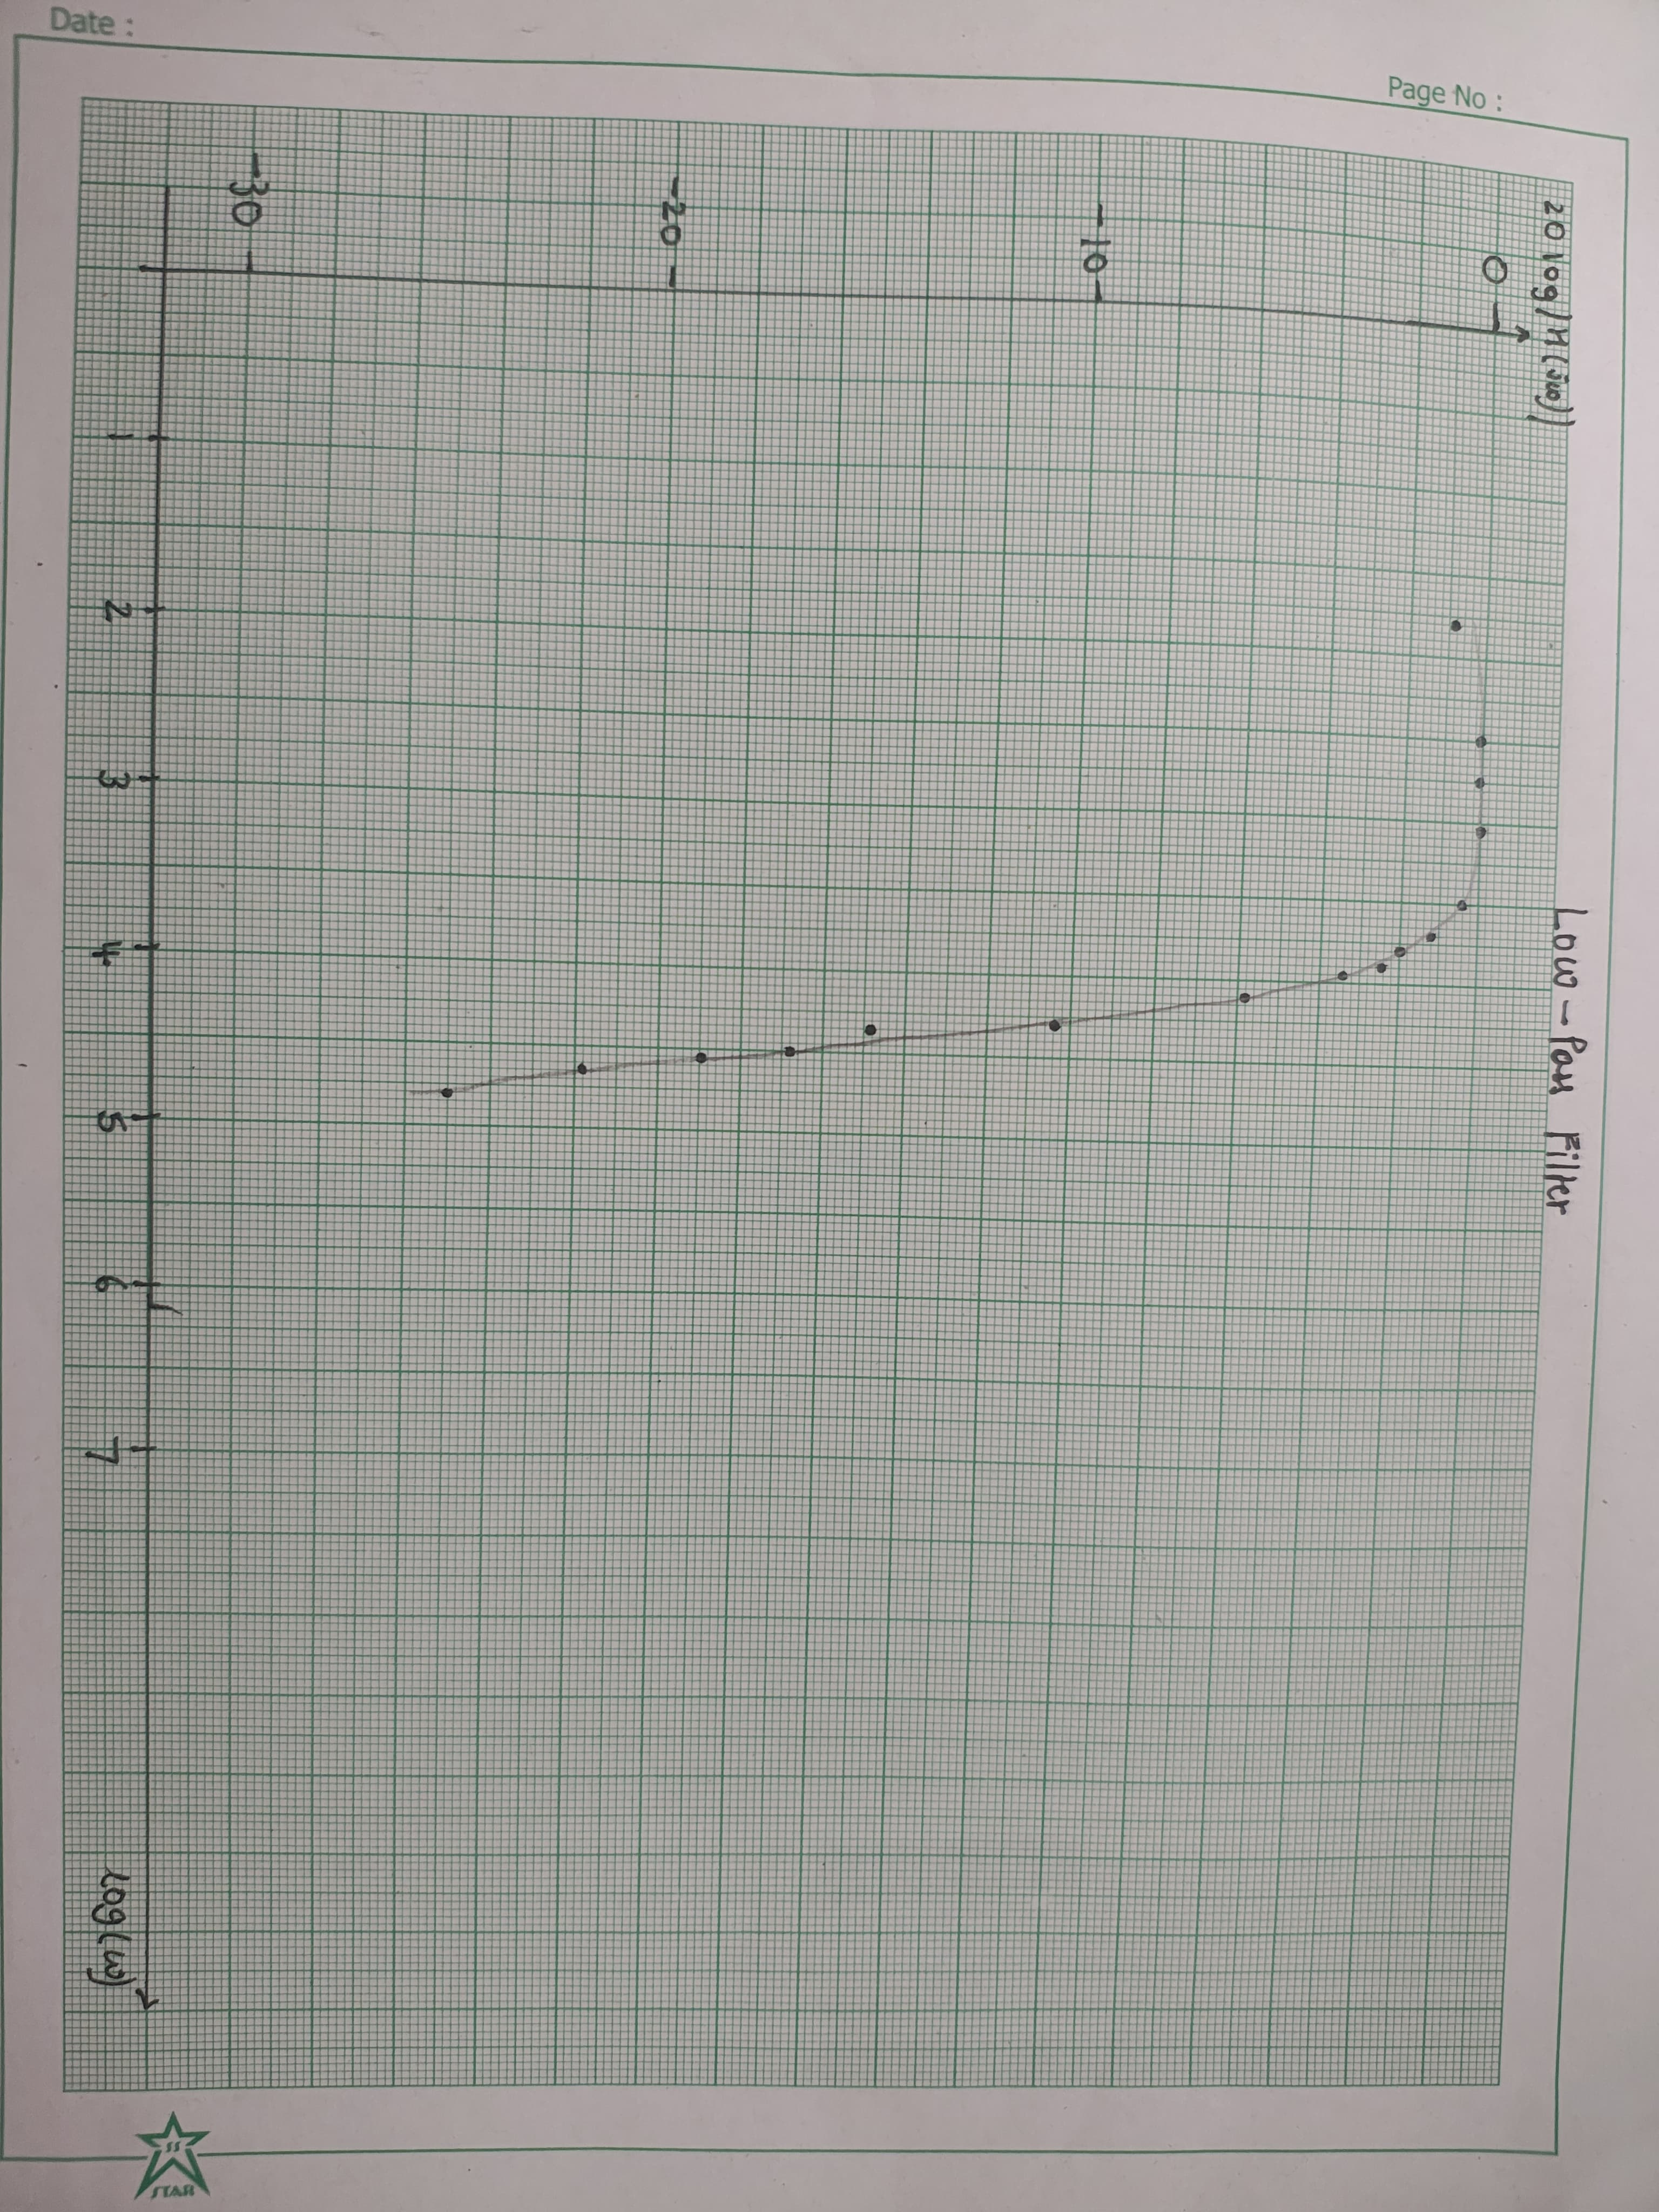
\includegraphics[ width=1\textwidth]{./Pictures/low_pass_bode.jpeg}}
    \caption{Bode Plot for Low-Pass Filter}
\end{figure*}
\FloatBarrier

\begin{figure*}[!htb]
    {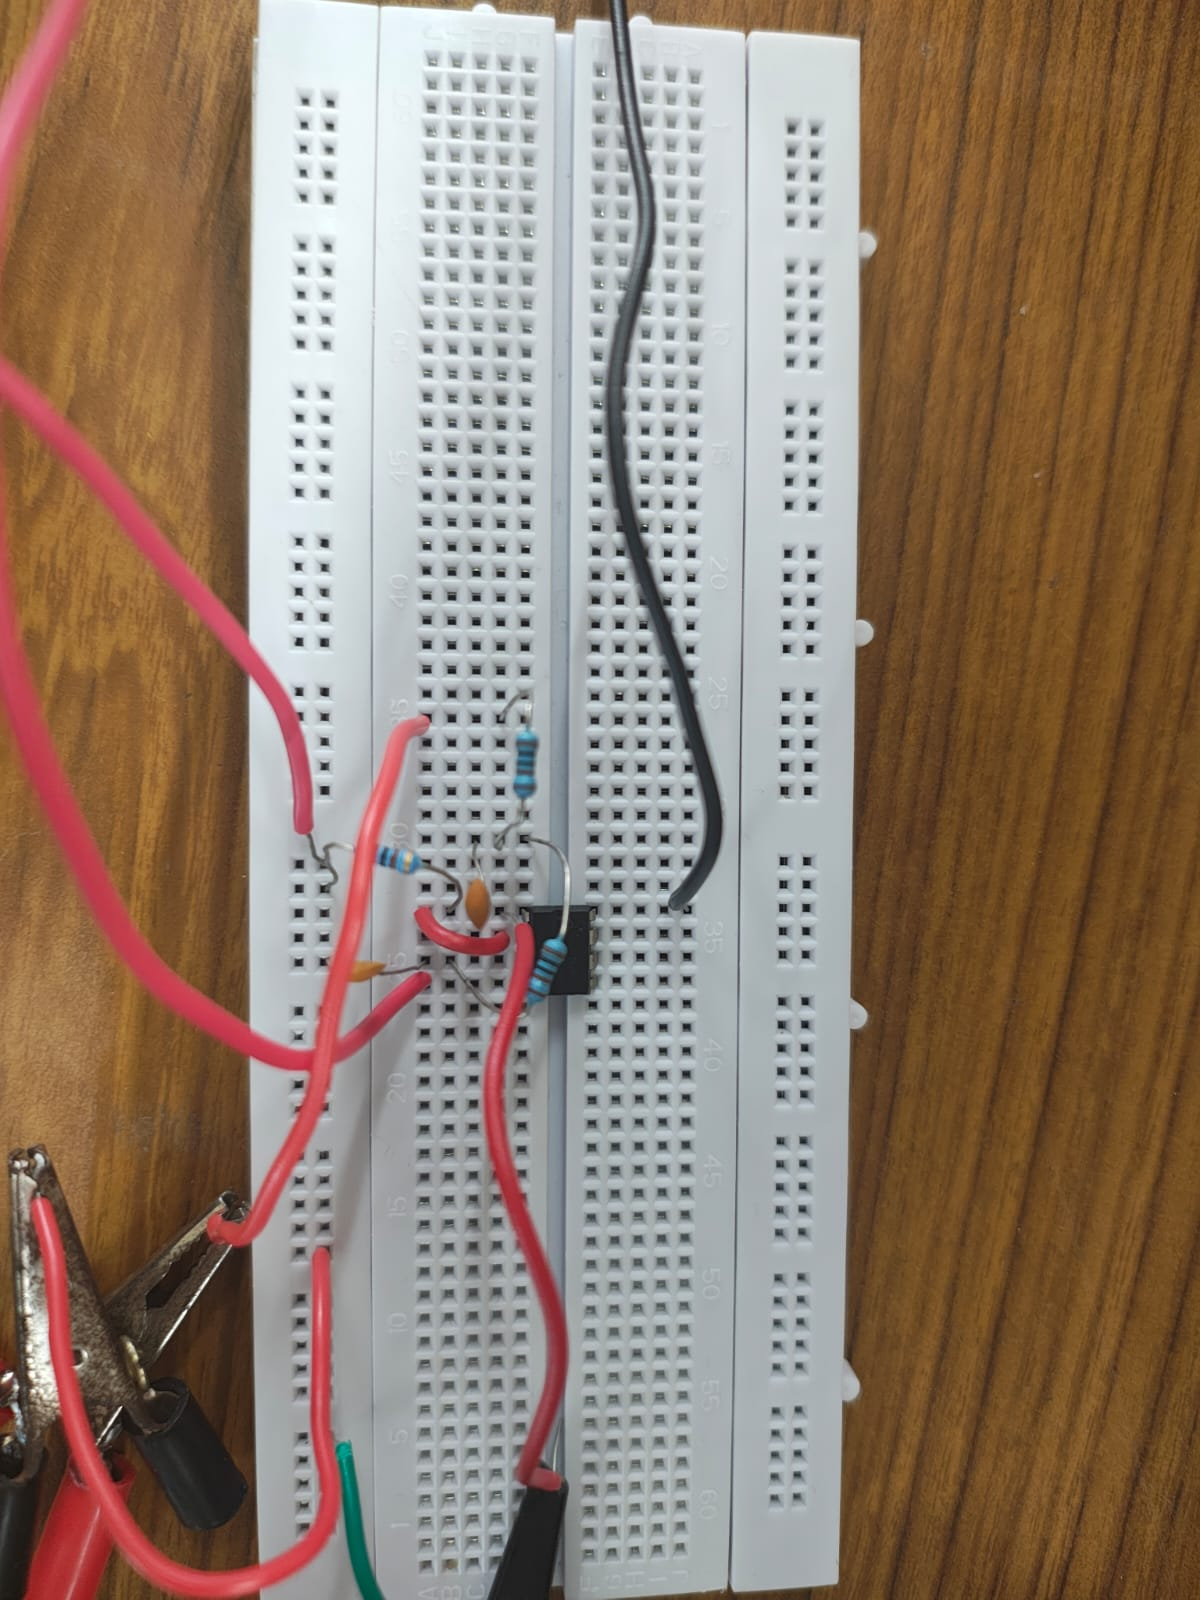
\includegraphics[ width=1\textwidth]{./Pictures/low_pass_circuit.jpeg}}
    \caption{Circuit for Low-Pass Filter}
\end{figure*}
\FloatBarrier

\begin{figure*}[!htb]
    {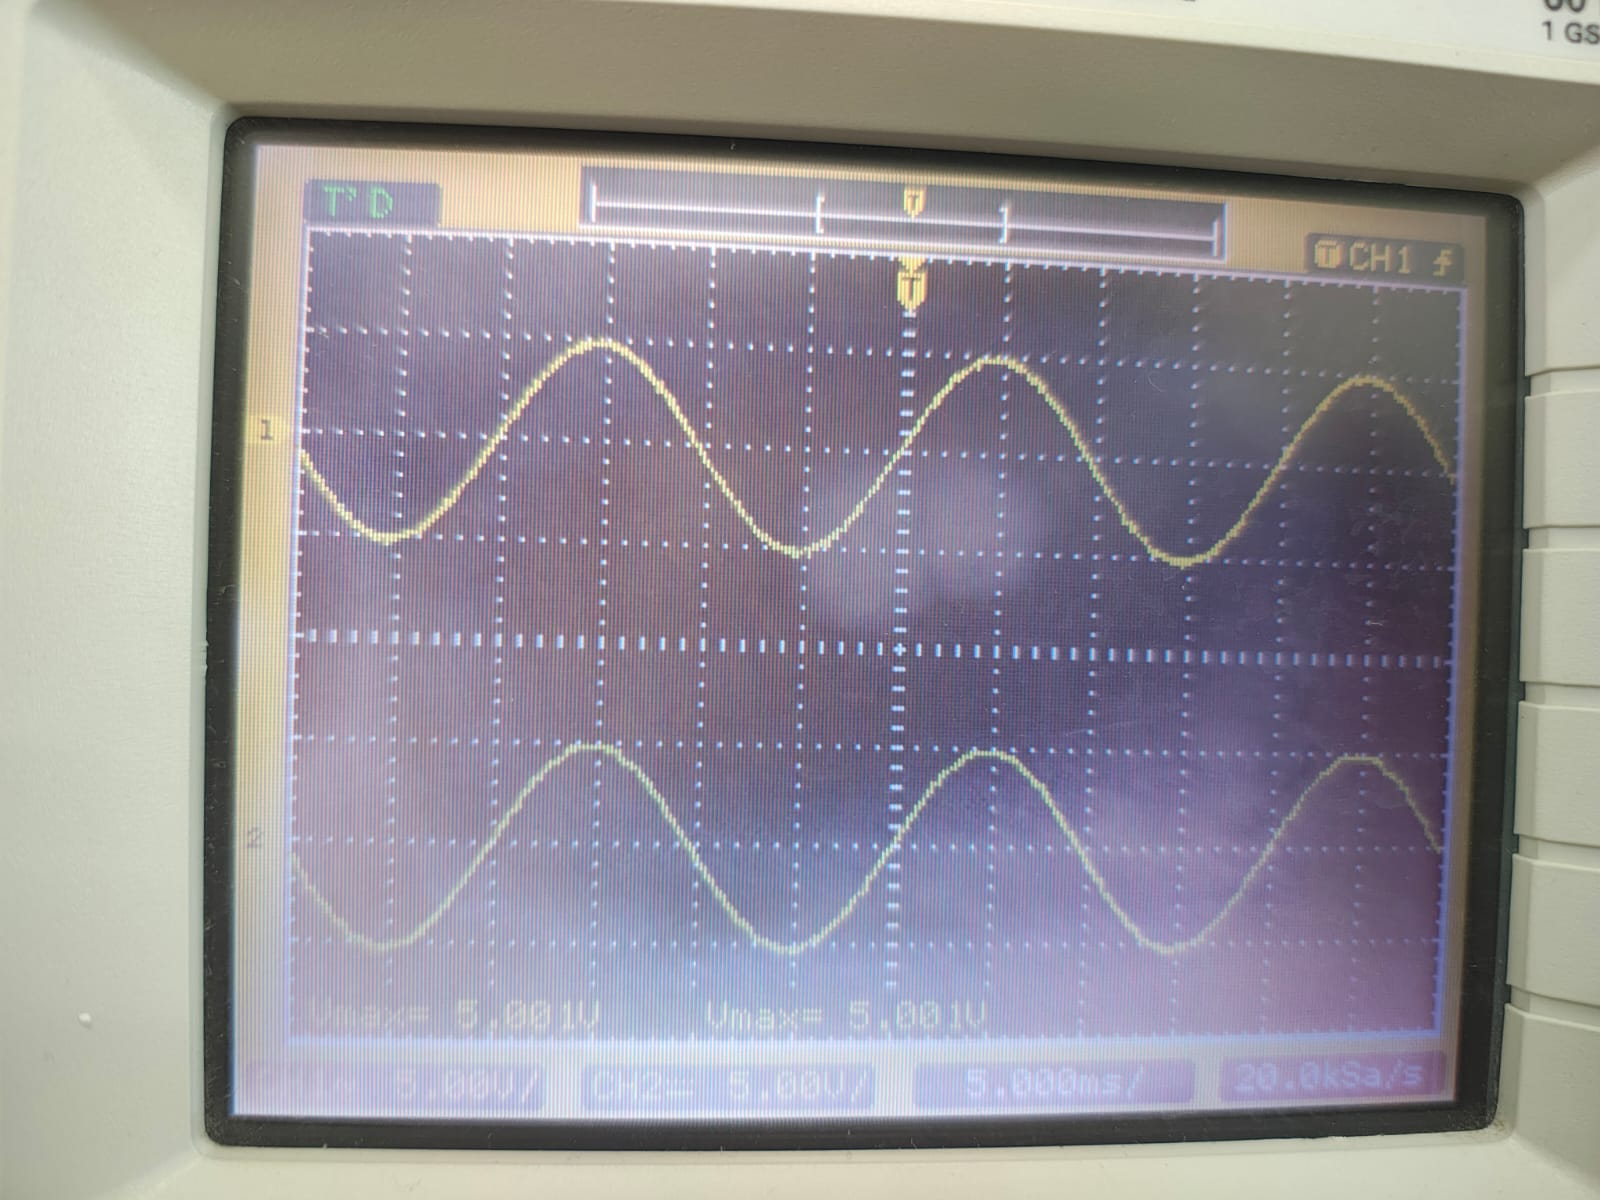
\includegraphics[ width=0.5\textwidth]{./Pictures/Lowpass/Lowpass1.jpeg}}
    \hspace{\fill}
    {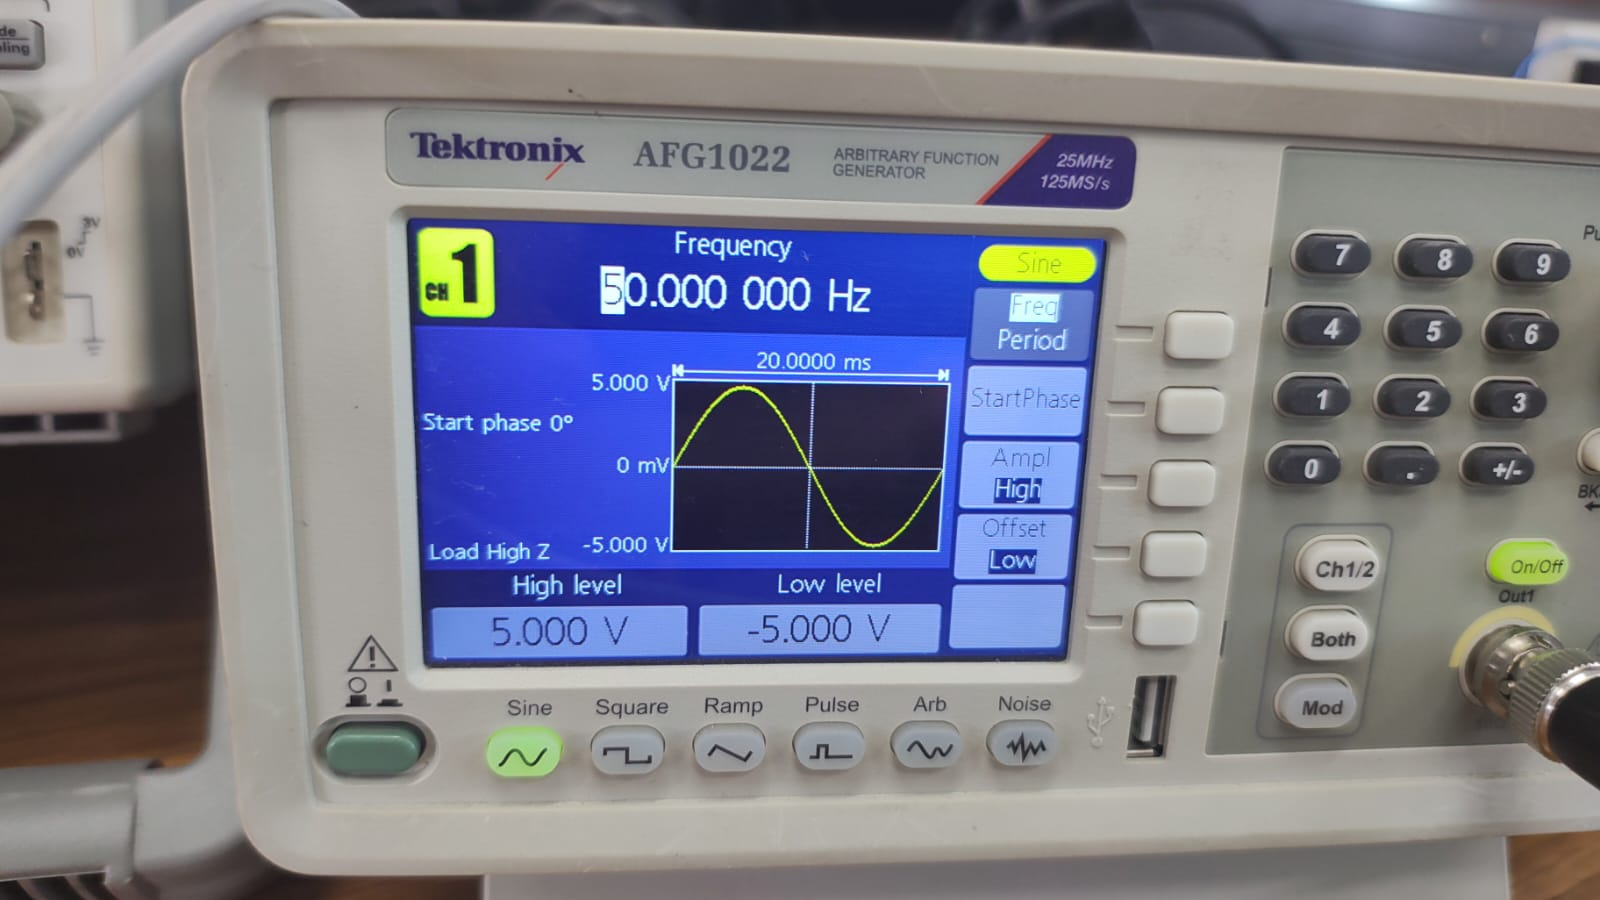
\includegraphics[ width=0.5\textwidth]{./Pictures/Lowpass/Lowpass3.jpeg}}
\end{figure*}
\FloatBarrier

\begin{figure*}[!htb]
    {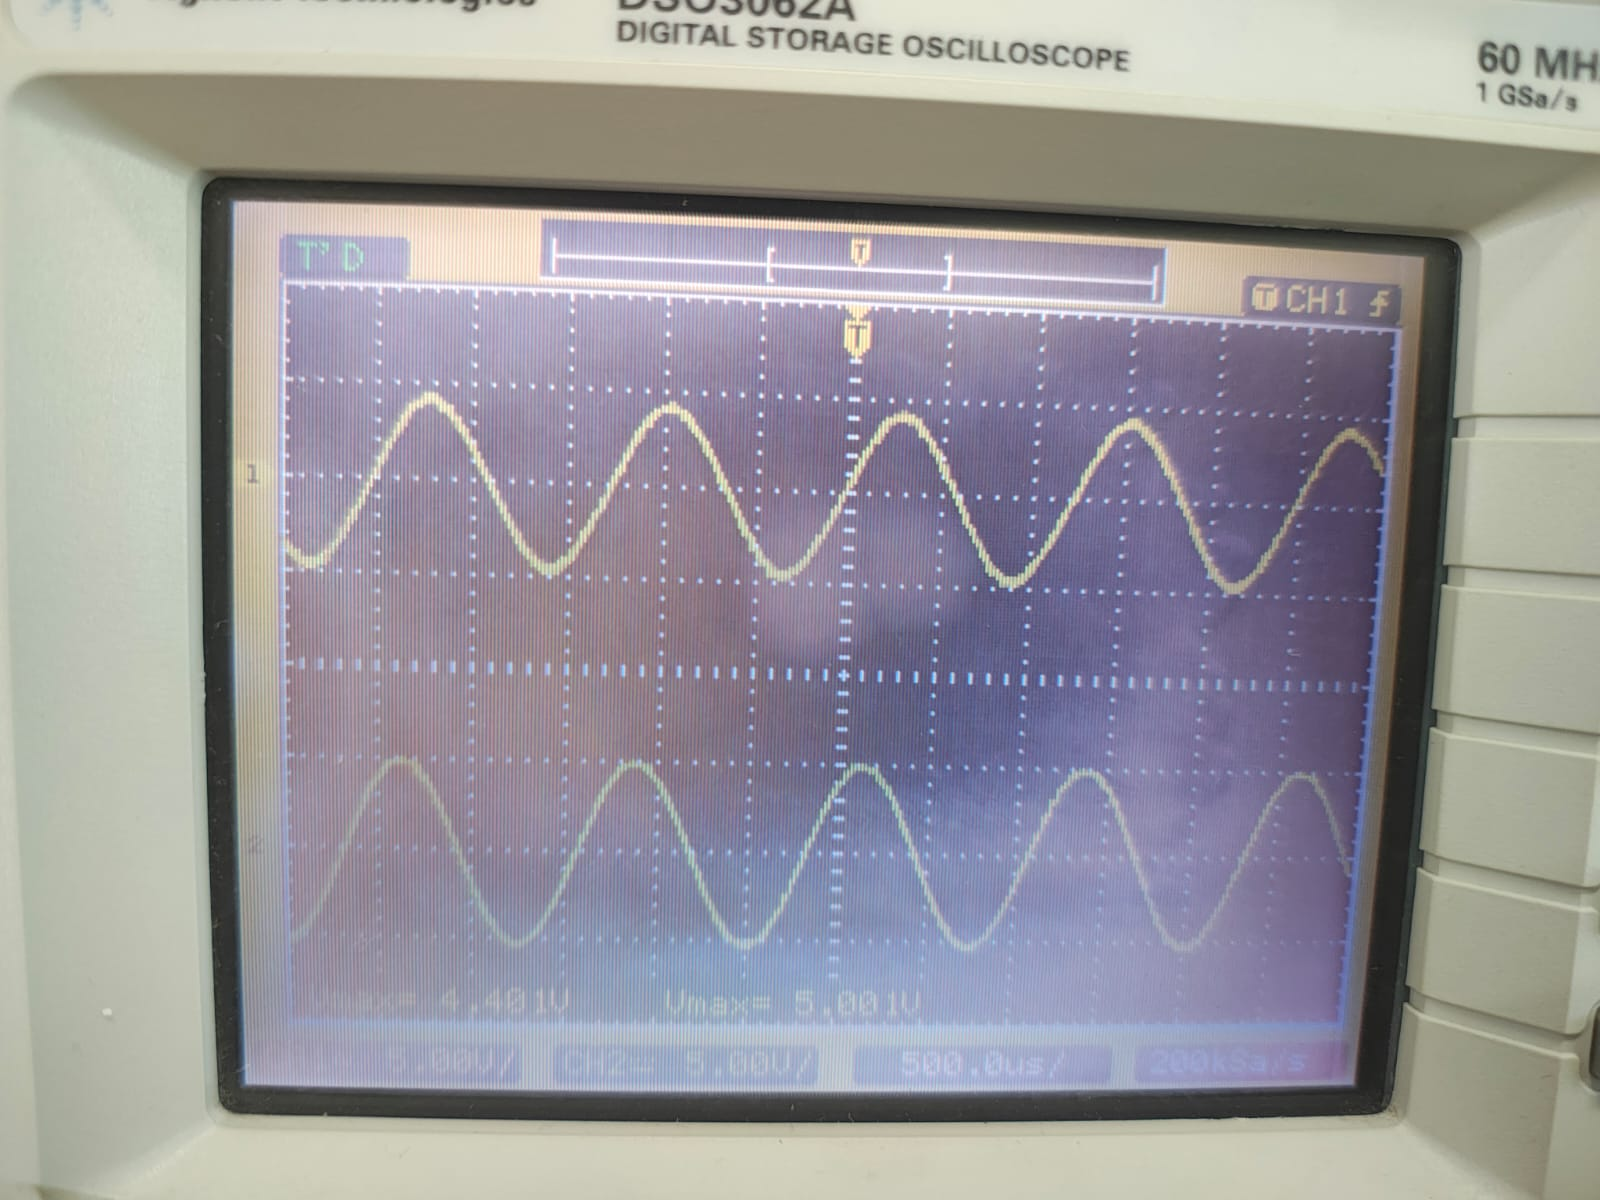
\includegraphics[ width=0.5\textwidth]{./Pictures/Lowpass/Lowpass11.jpeg}}
    \hspace{\fill}
    {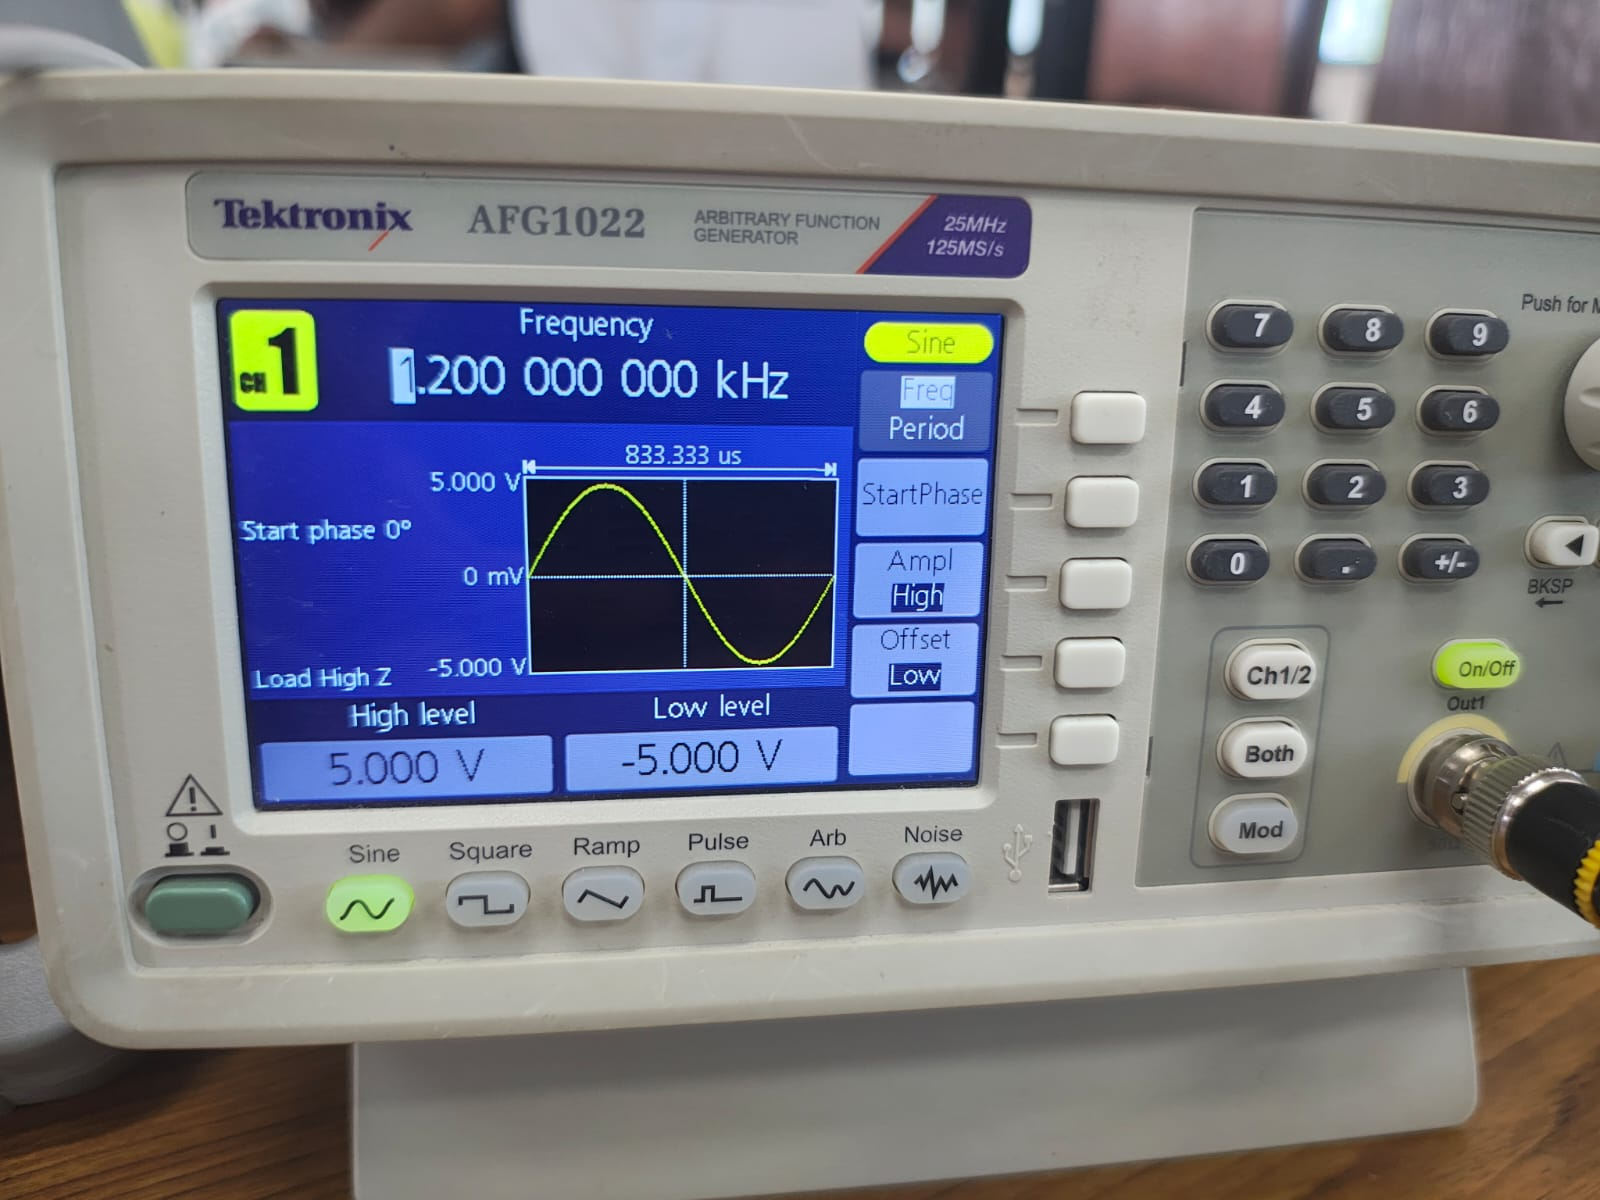
\includegraphics[ width=0.5\textwidth]{./Pictures/Lowpass/Lowpass12.jpeg}}
\end{figure*}
\FloatBarrier

\begin{figure*}[!htb]
    {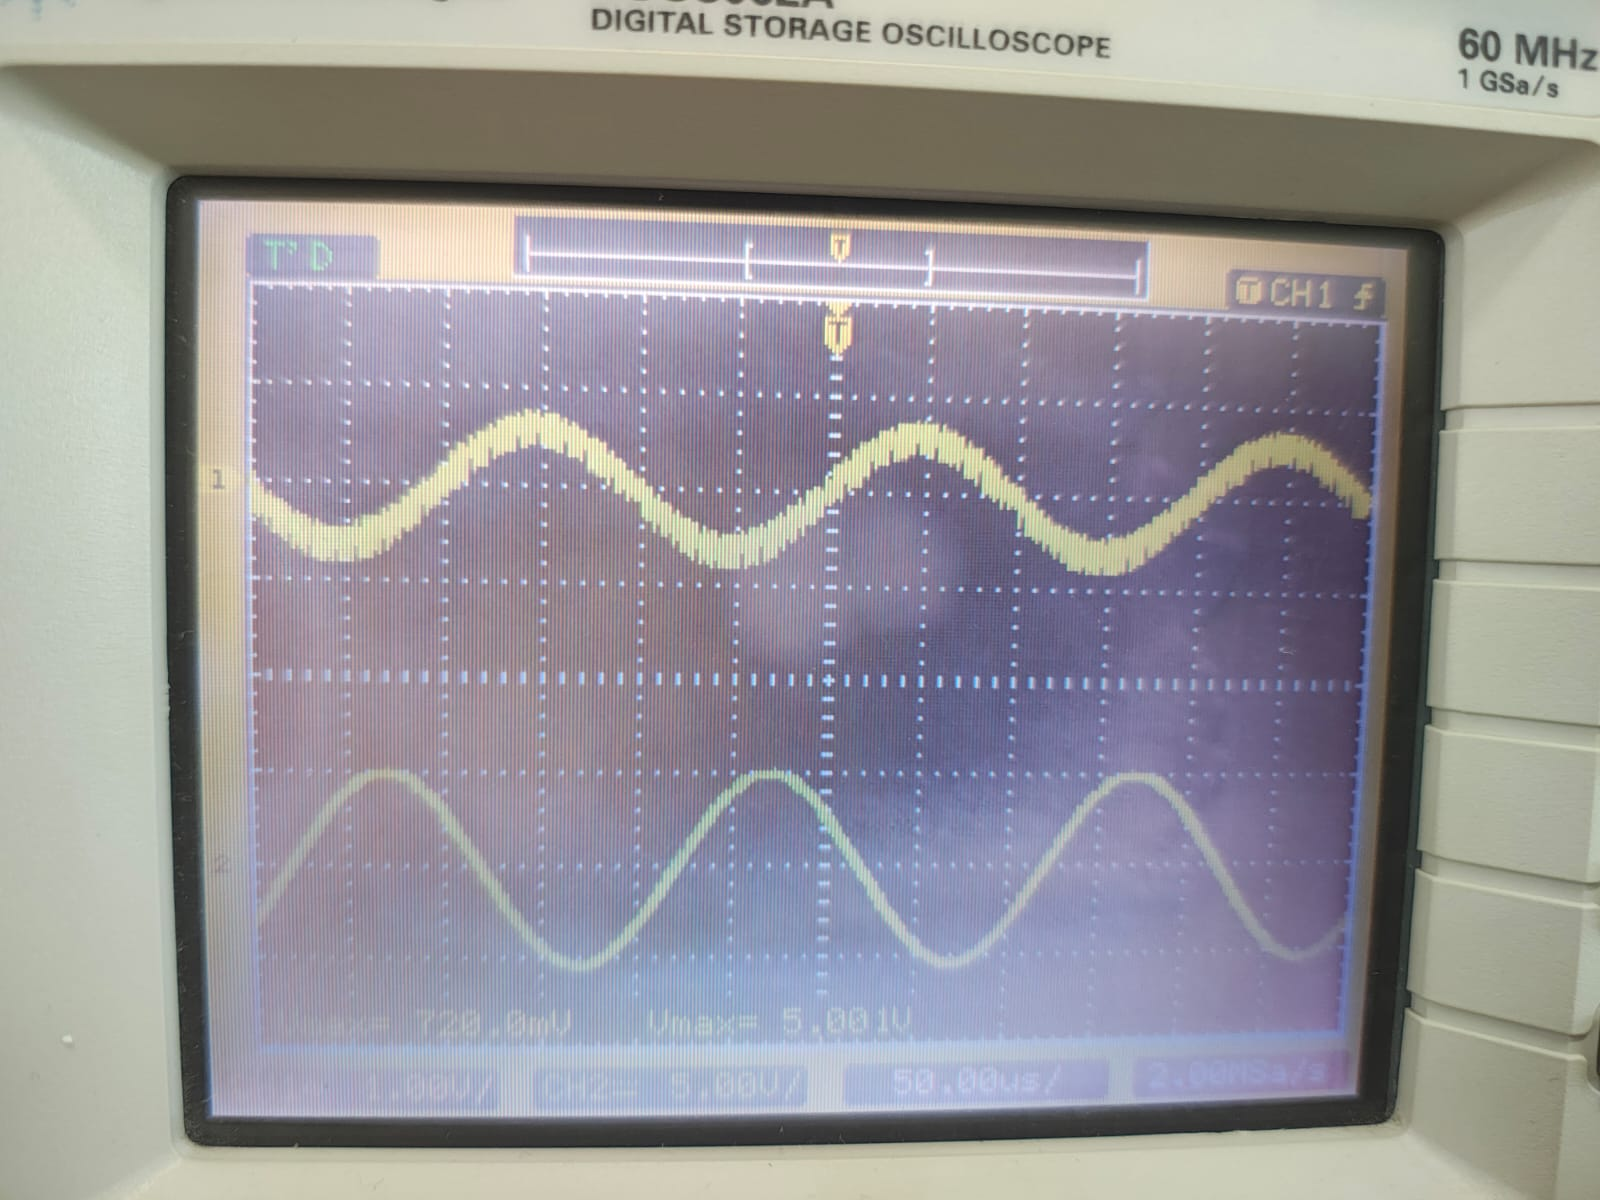
\includegraphics[ width=0.5\textwidth]{./Pictures/Lowpass/Lowpass23.jpeg}}
    \hspace{\fill}
    {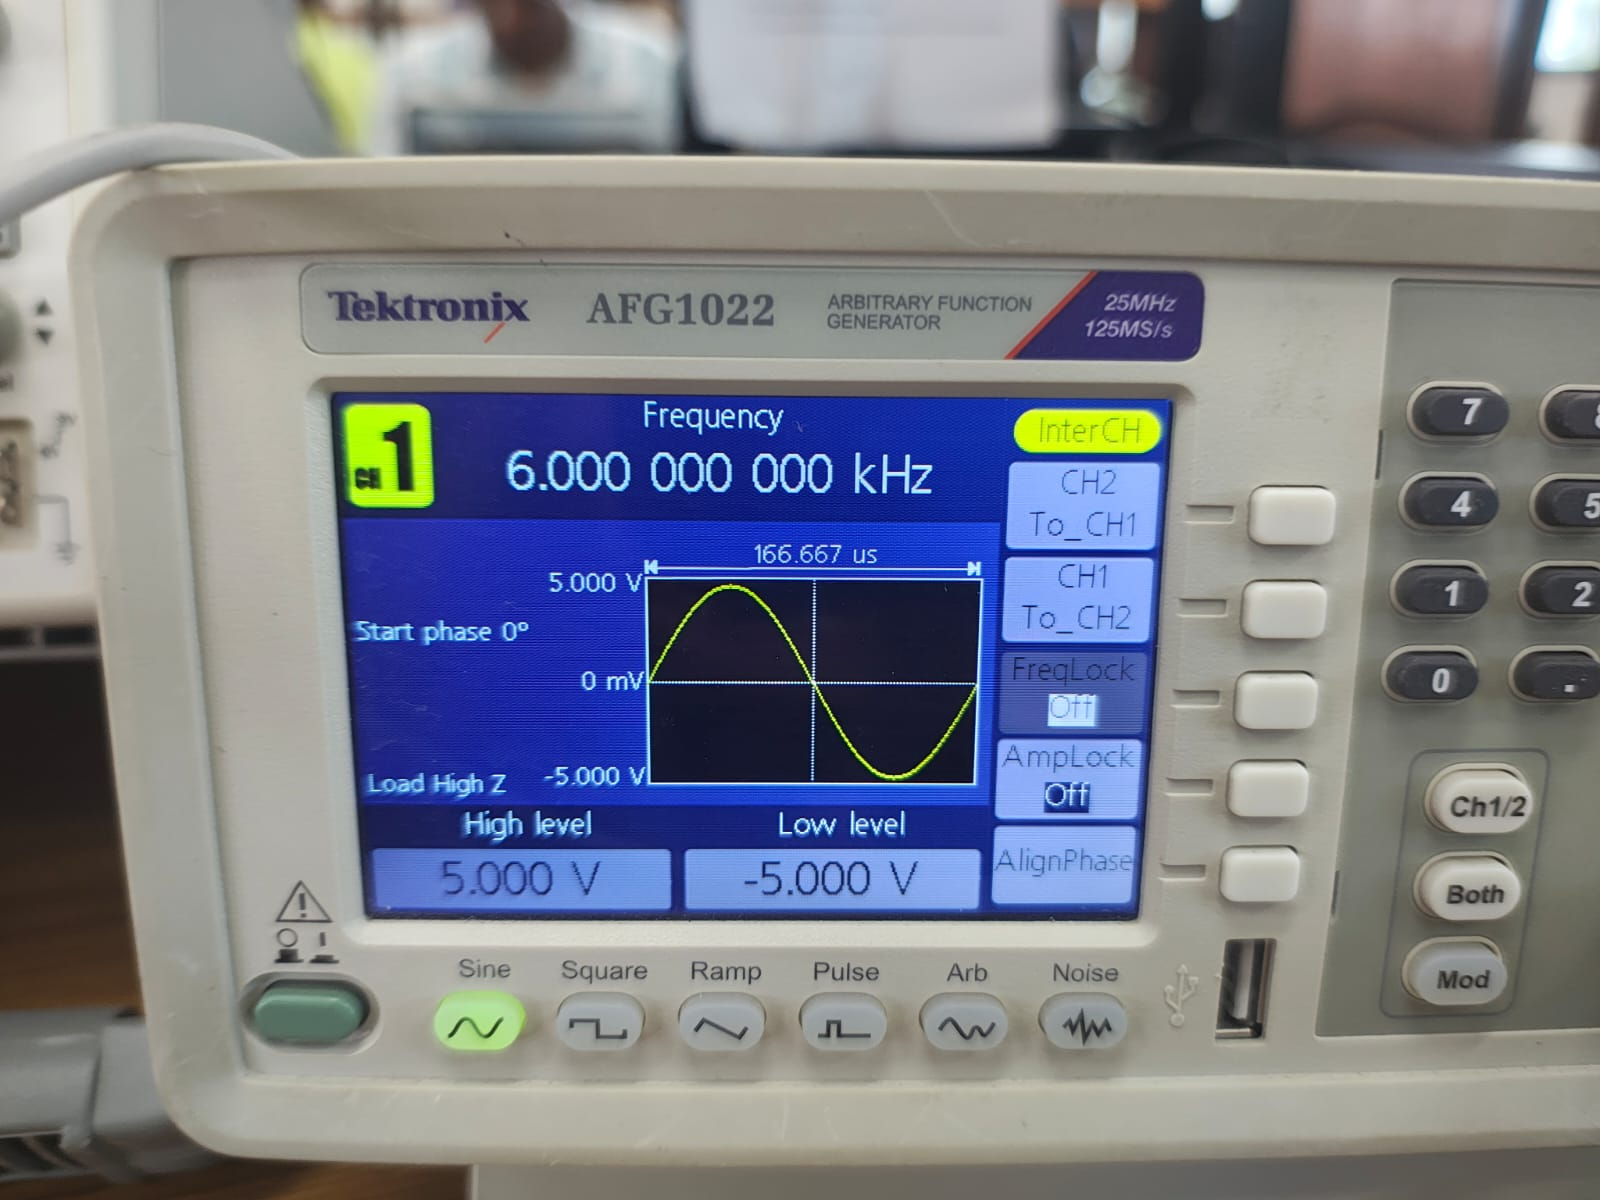
\includegraphics[ width=0.5\textwidth]{./Pictures/Lowpass/Lowpass24.jpeg}}
\end{figure*}
\FloatBarrier

\subsection{High-Pass Filter}
\begin{align*}
    R = 1k\Omega, C = 220nF
\end{align*}

\begin{table}[h]
\centering
\begin{tabular}{|c|c|}
\hline
$\log(\omega)$ & $20 \log(|H(s)|)$ \\
\hline
3.0992 & -20.3546 \\
3.2753 & -15.4938 \\
3.4971 & -9.4680 \\
3.5763 & -7.2863 \\
3.6433 & -6.0869 \\
3.7982 & -3.6593 \\
4.0992 & -1.9360 \\
4.4971 & -1.1084 \\
4.7982 & -1.1084 \\
\hline
\end{tabular}
\caption{Logarithmic frequency response data for high-pass filter}
\label{tab:freq_response}
\end{table}
\FloatBarrier

\begin{figure*}[!htb]
    {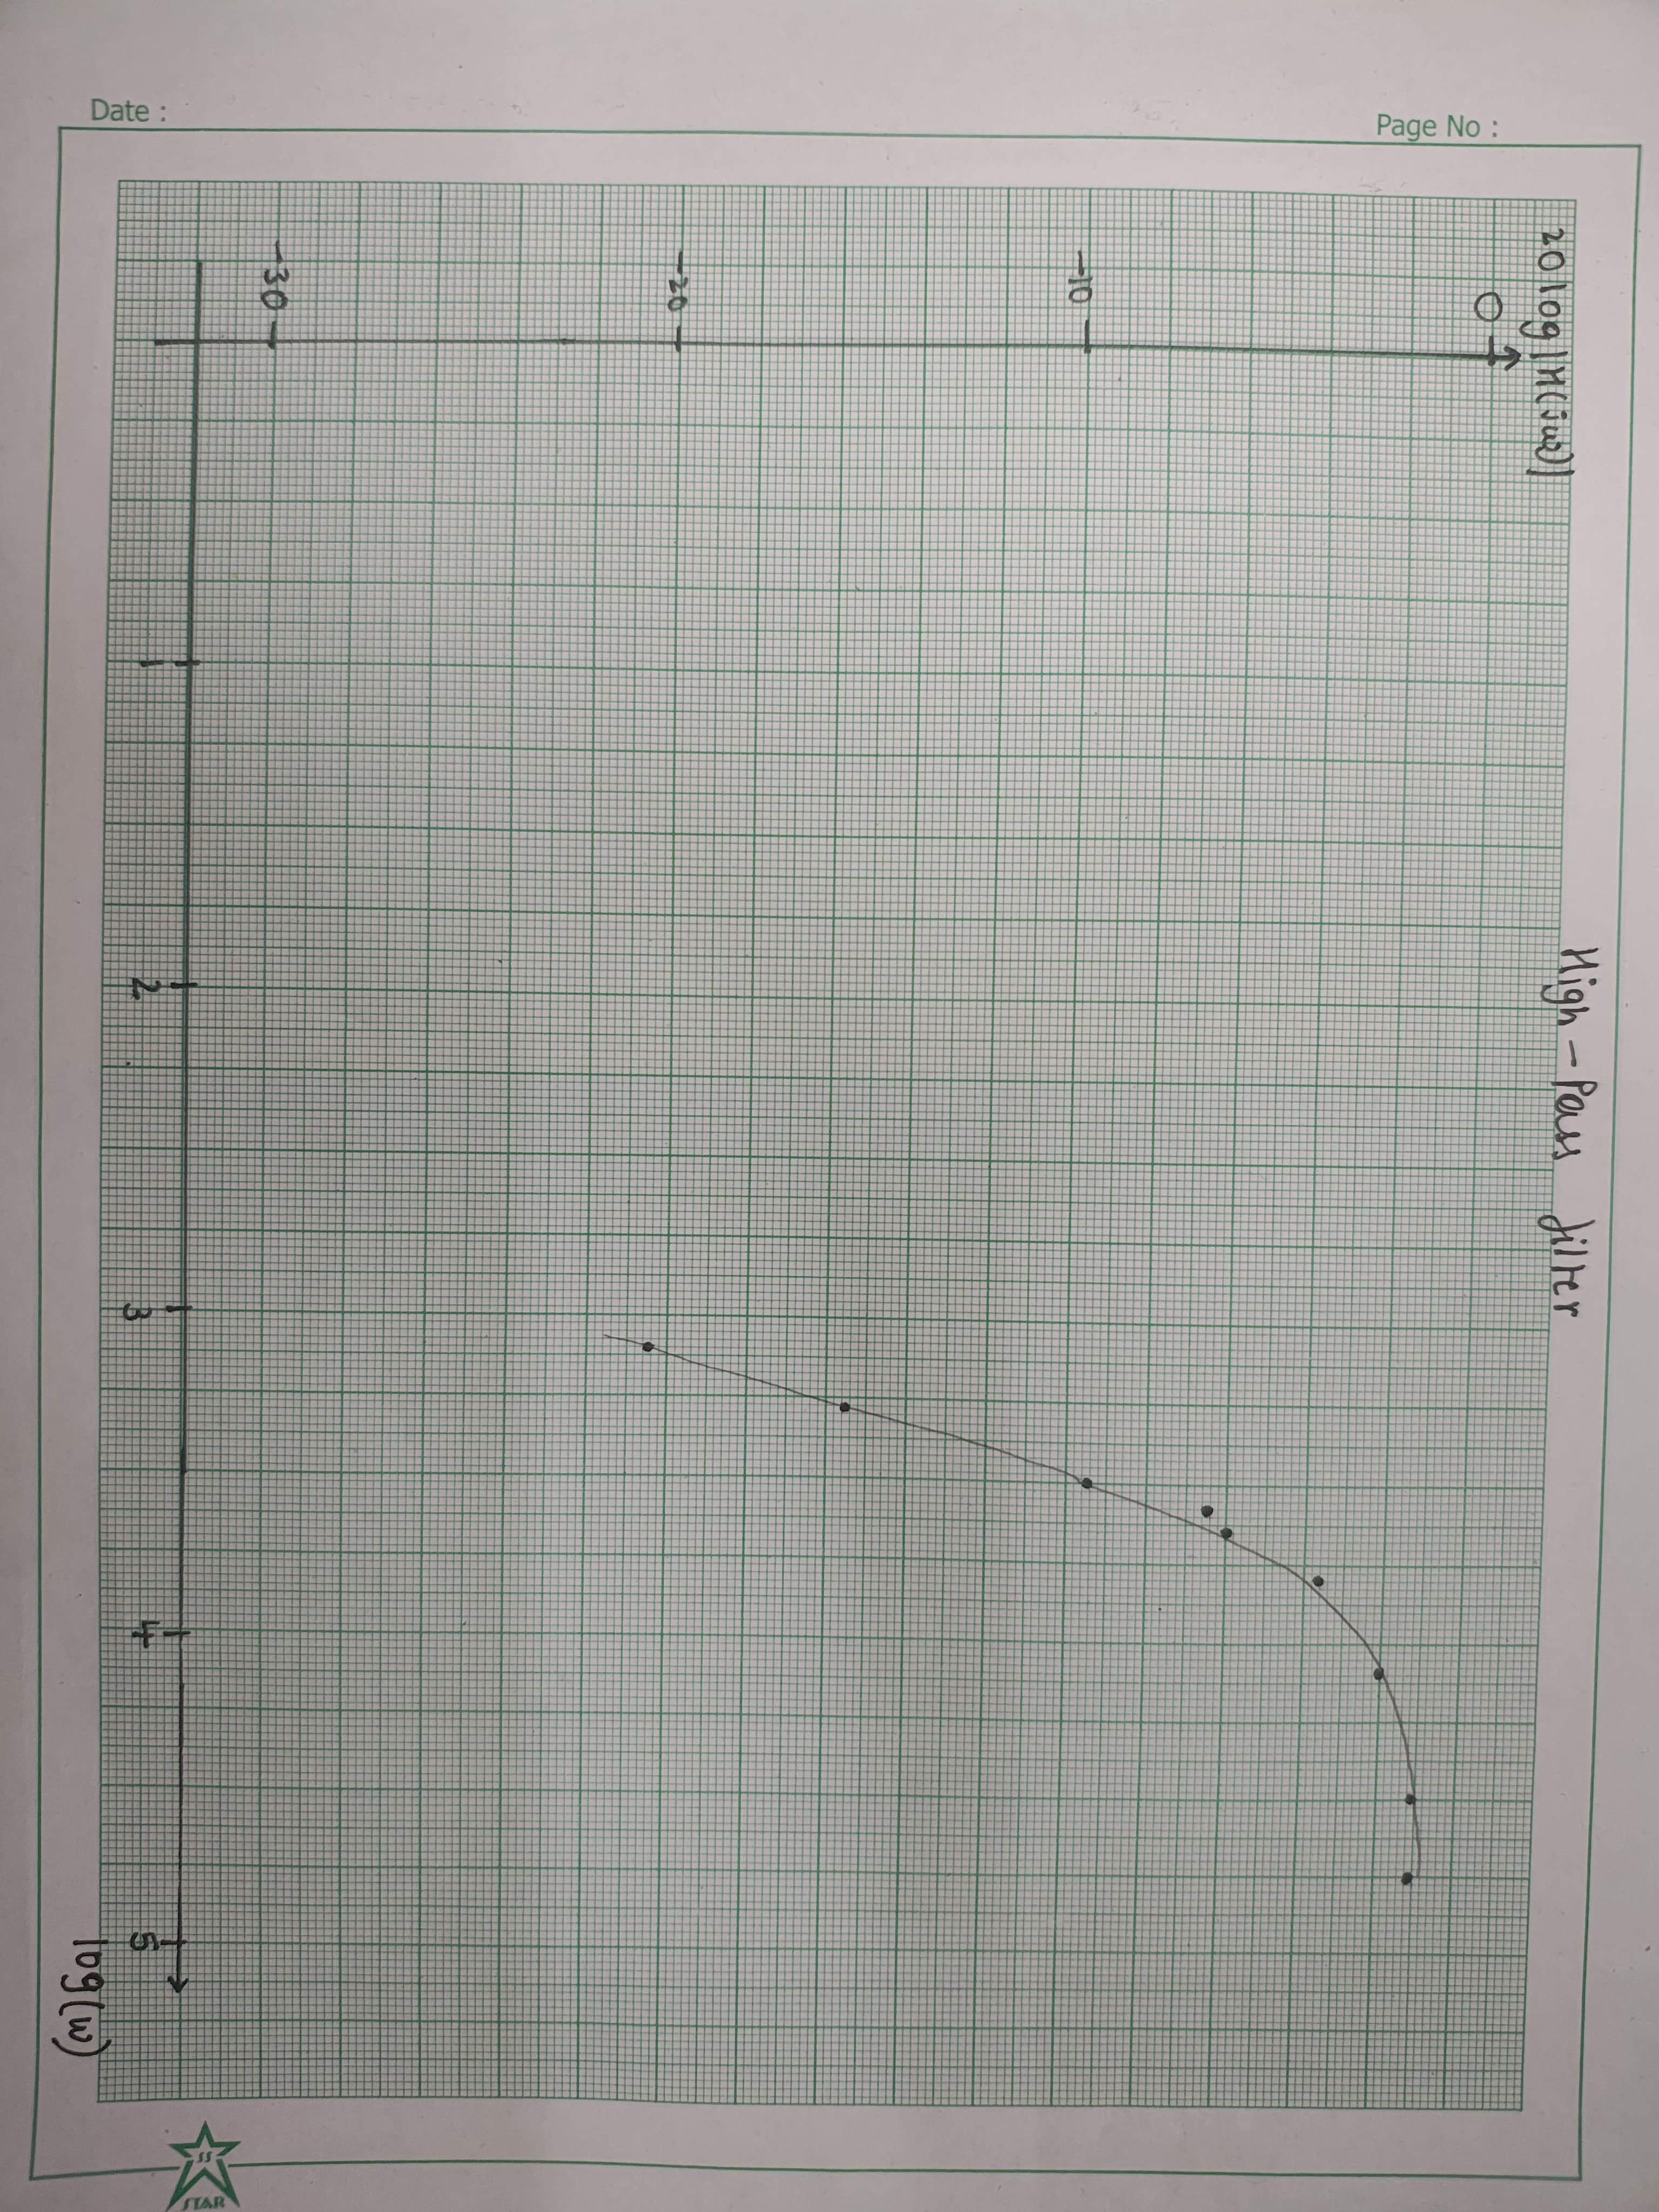
\includegraphics[ width=1\textwidth]{./Pictures/high_pass_bode.jpeg}}
    \caption{Bode Plot for High-Pass Filter}
\end{figure*}
\FloatBarrier

\begin{figure*}[!htb]
    {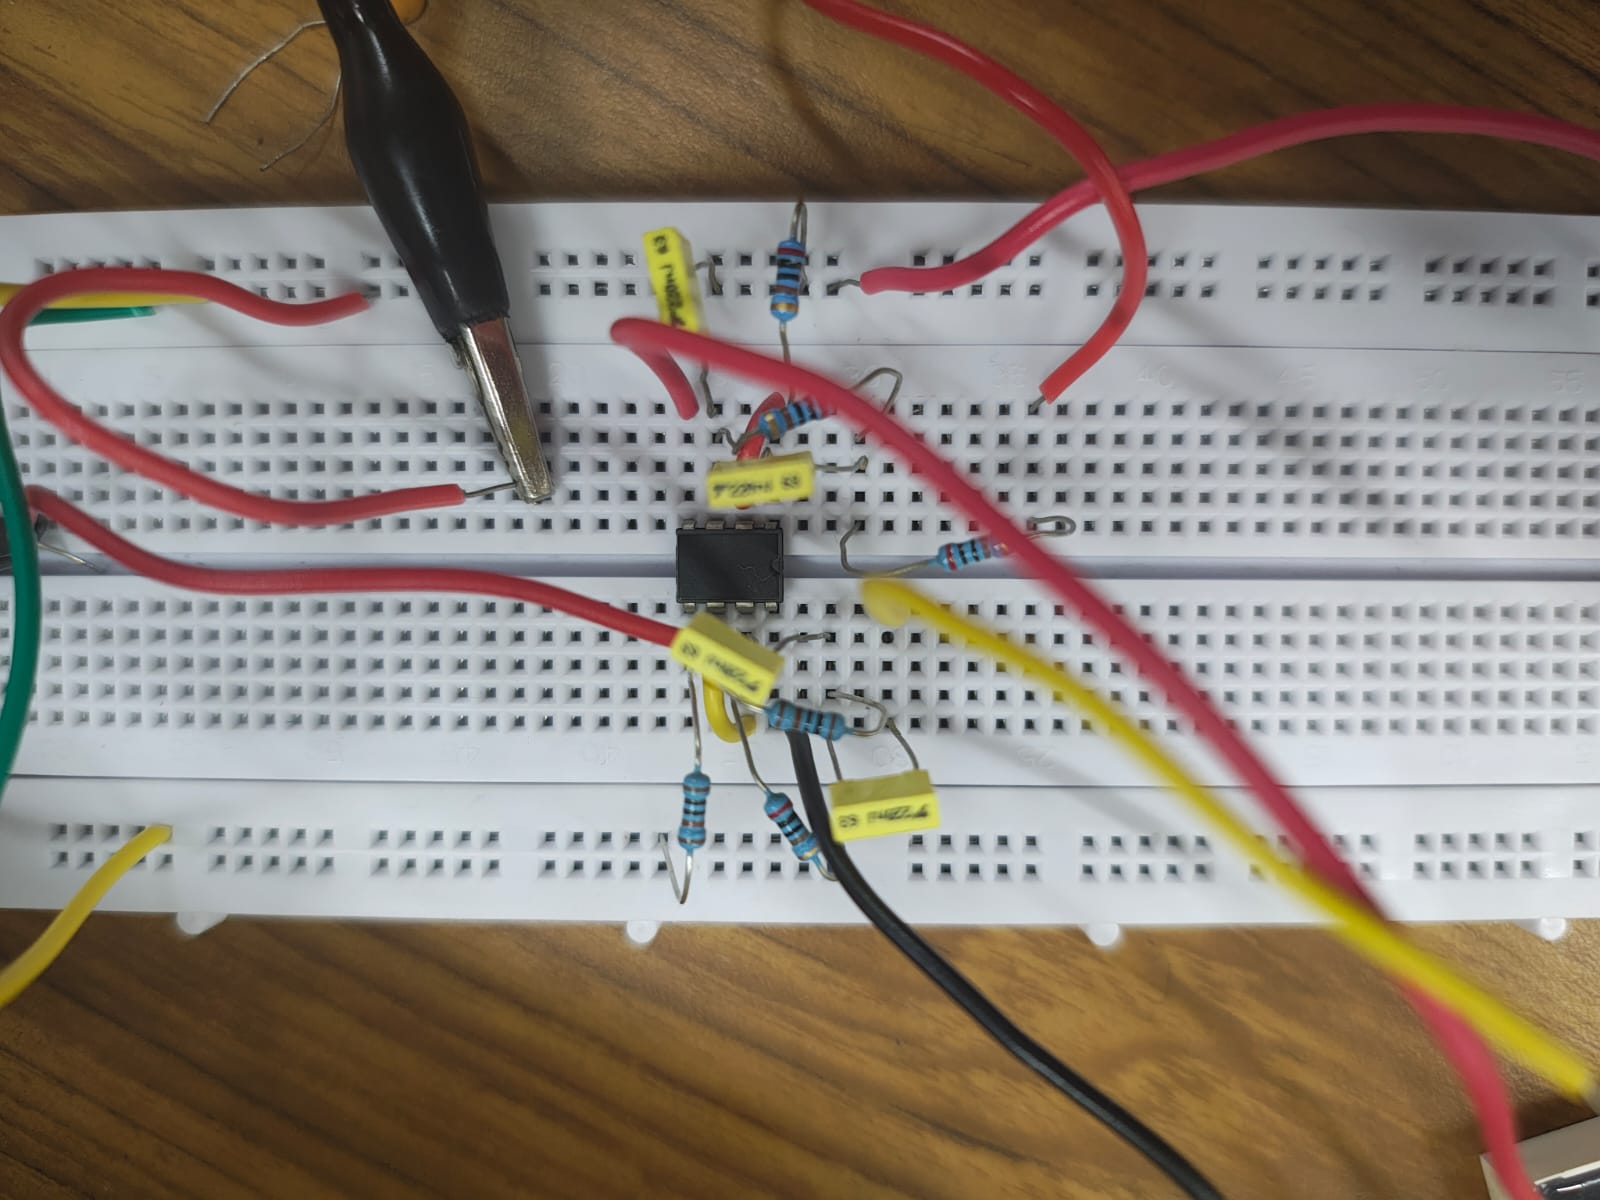
\includegraphics[ width=1\textwidth]{./Pictures/high_pass_circuit.jpeg}}
    \caption{Circuit for High-Pass Filter}
\end{figure*}
\FloatBarrier

\begin{figure*}[!htb]
    {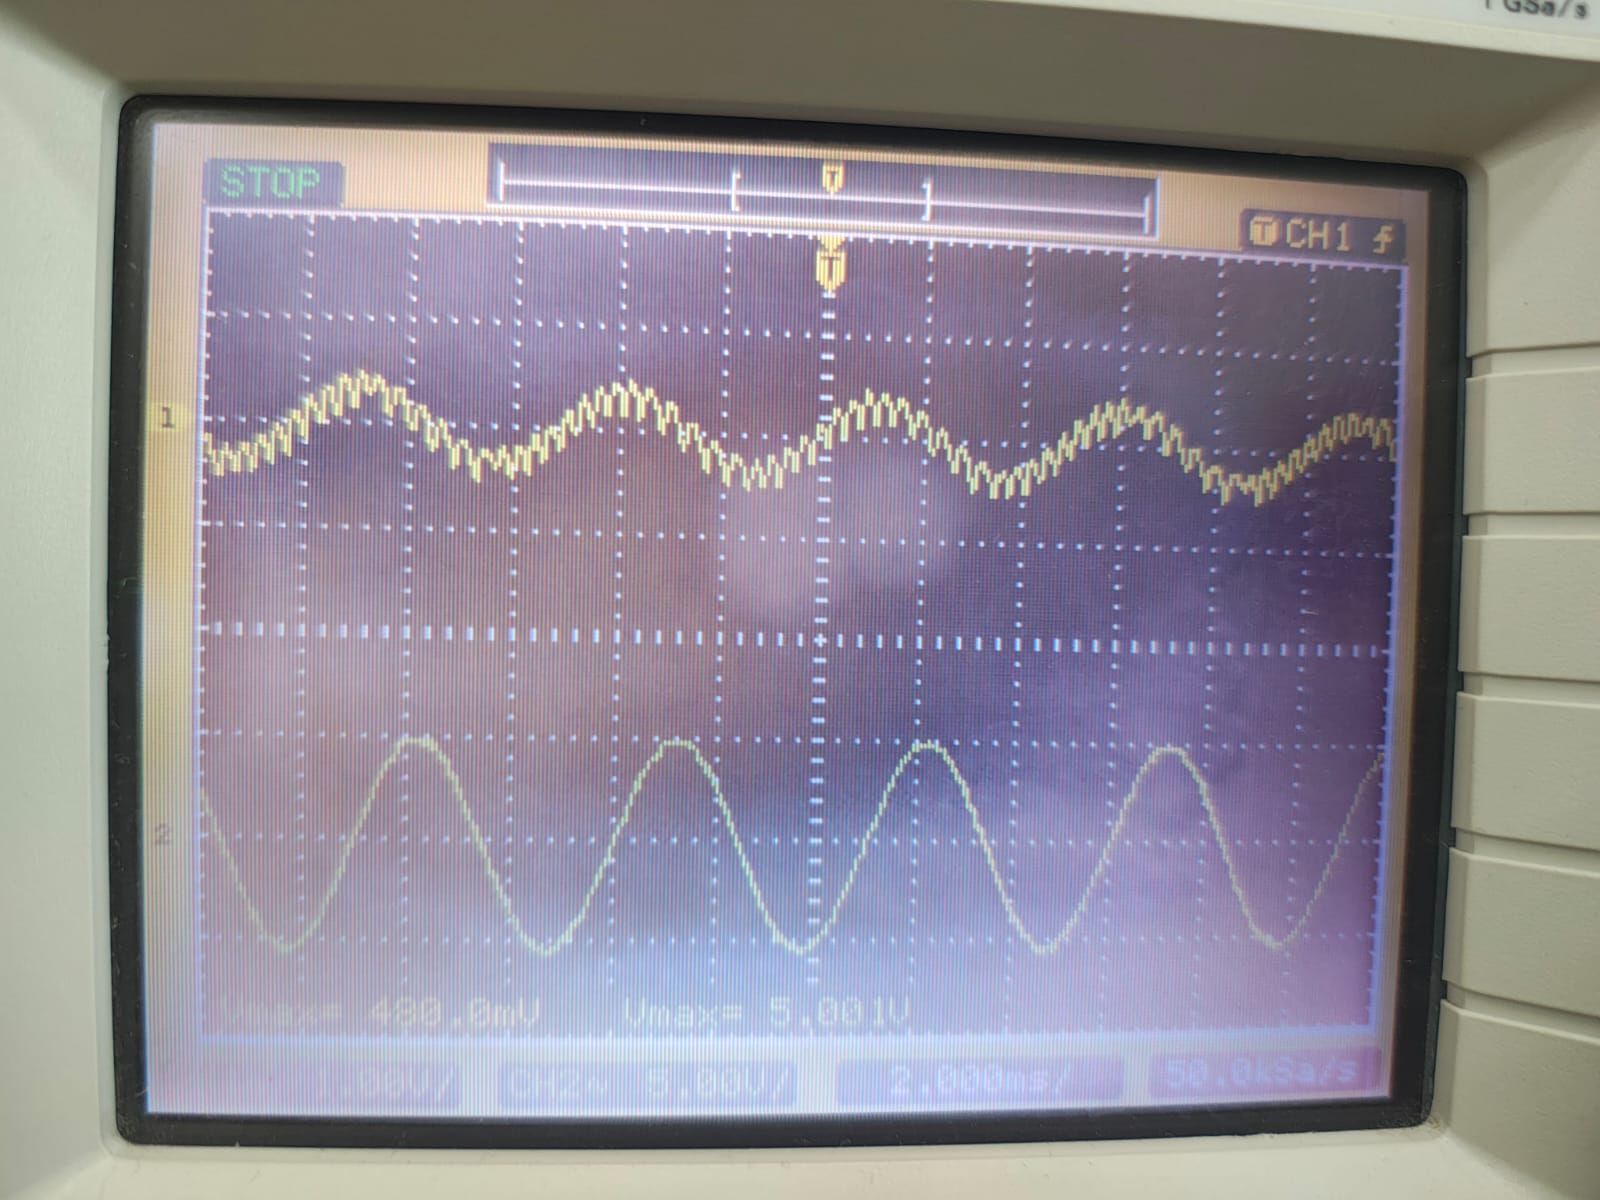
\includegraphics[ width=0.5\textwidth]{./Pictures/Highpass/Highpass3.jpeg}}
    \hspace{\fill}
    {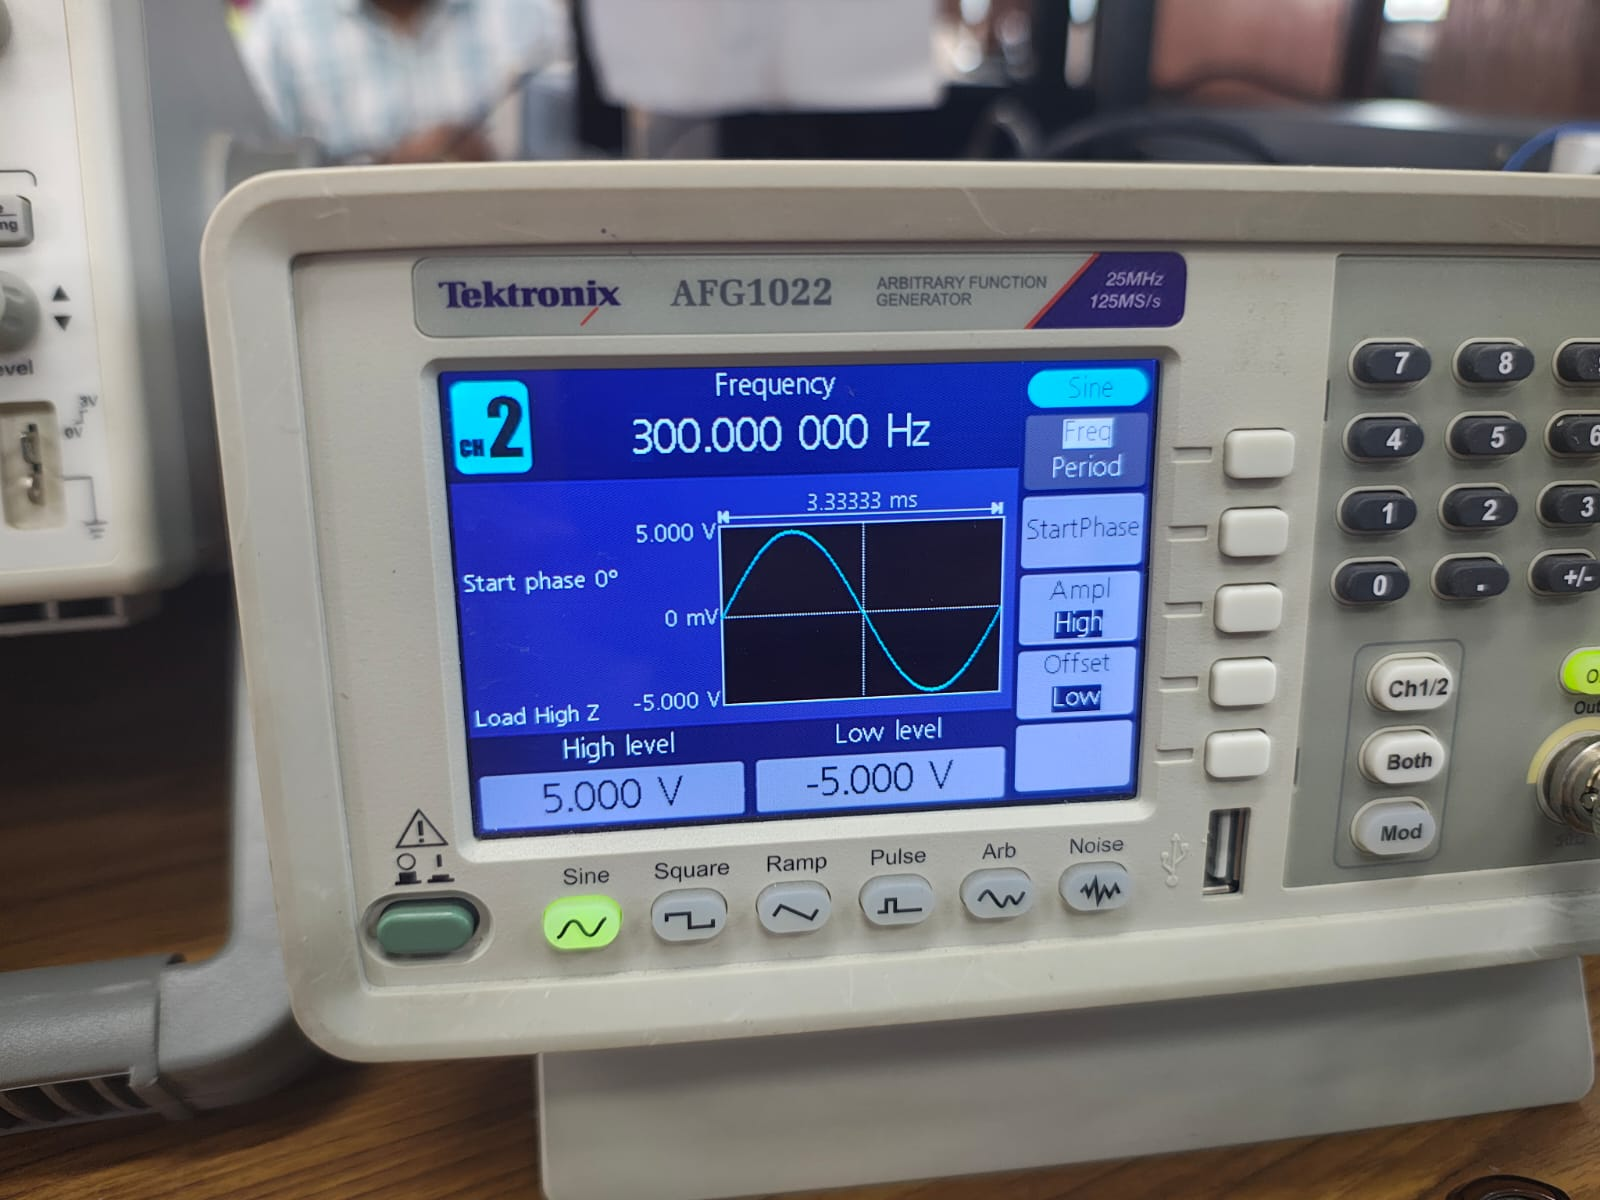
\includegraphics[ width=0.5\textwidth]{./Pictures/Highpass/Highpass4.jpeg}}
\end{figure*}
\FloatBarrier

\begin{figure*}[!htb]
    {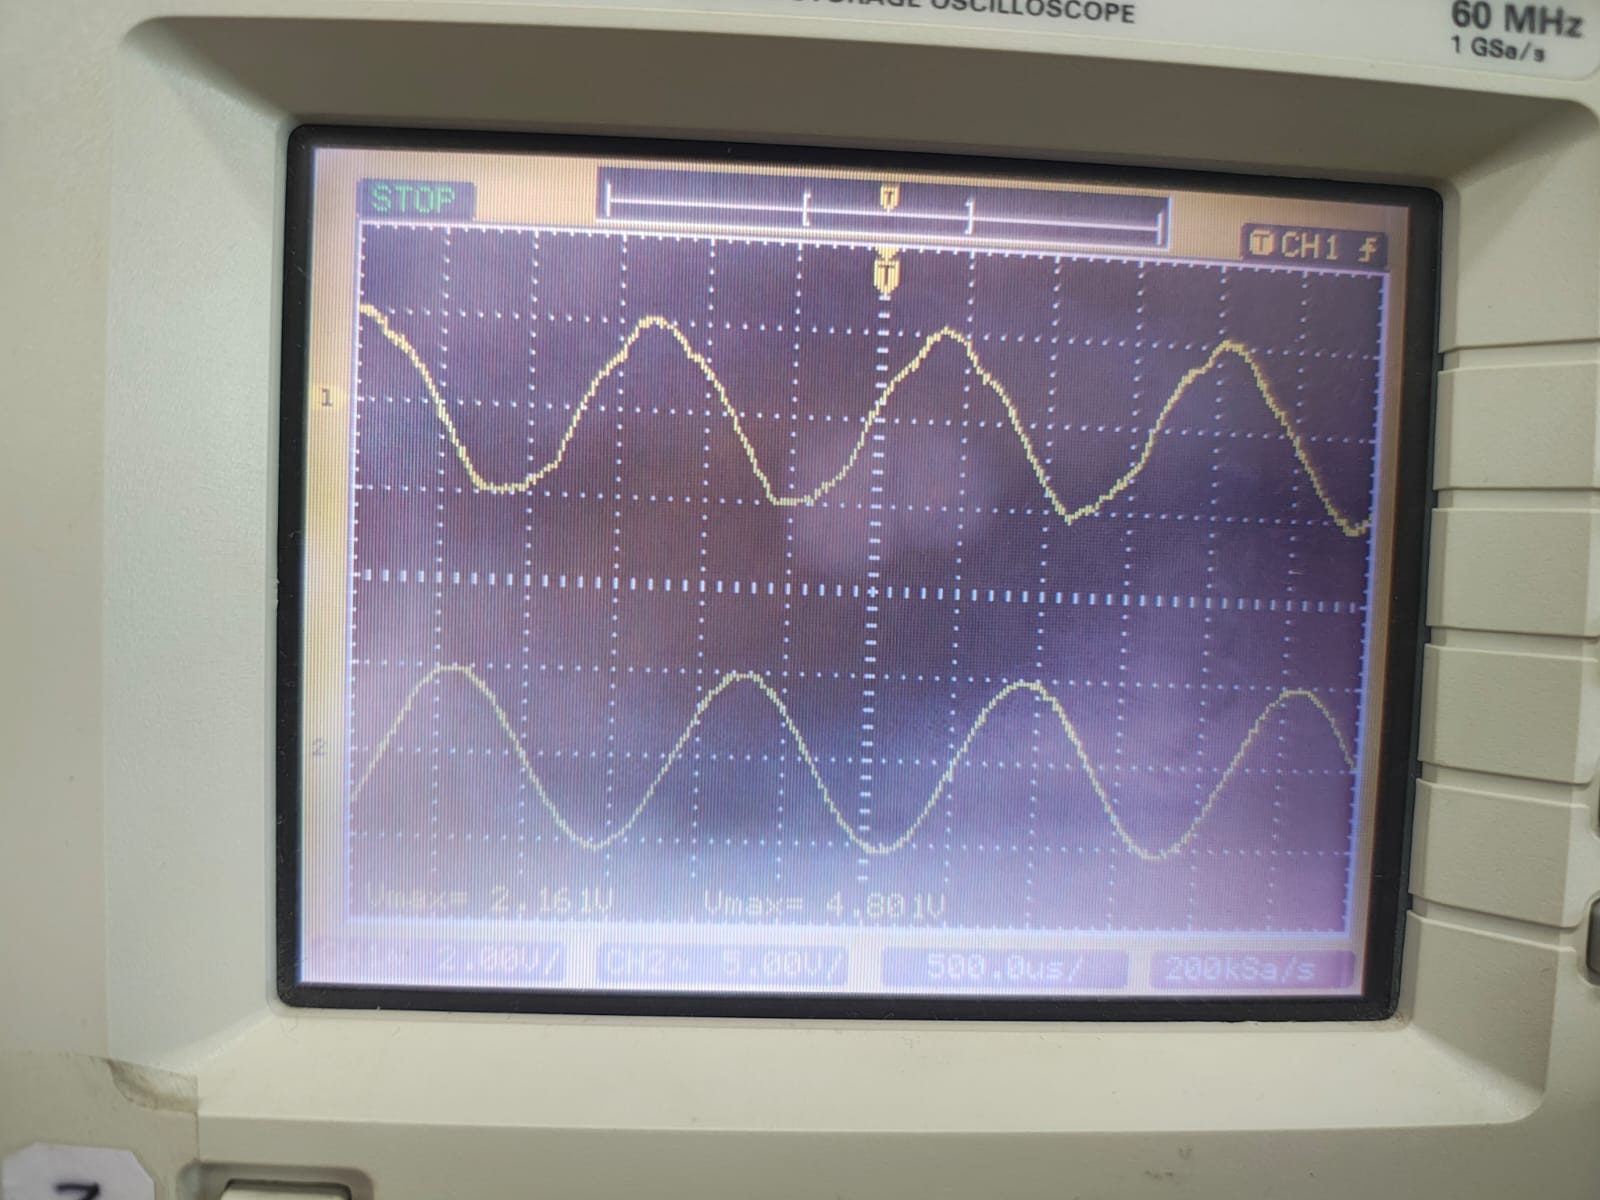
\includegraphics[ width=0.5\textwidth]{./Pictures/Highpass/Highpass11.jpeg}}
    \hspace{\fill}
    {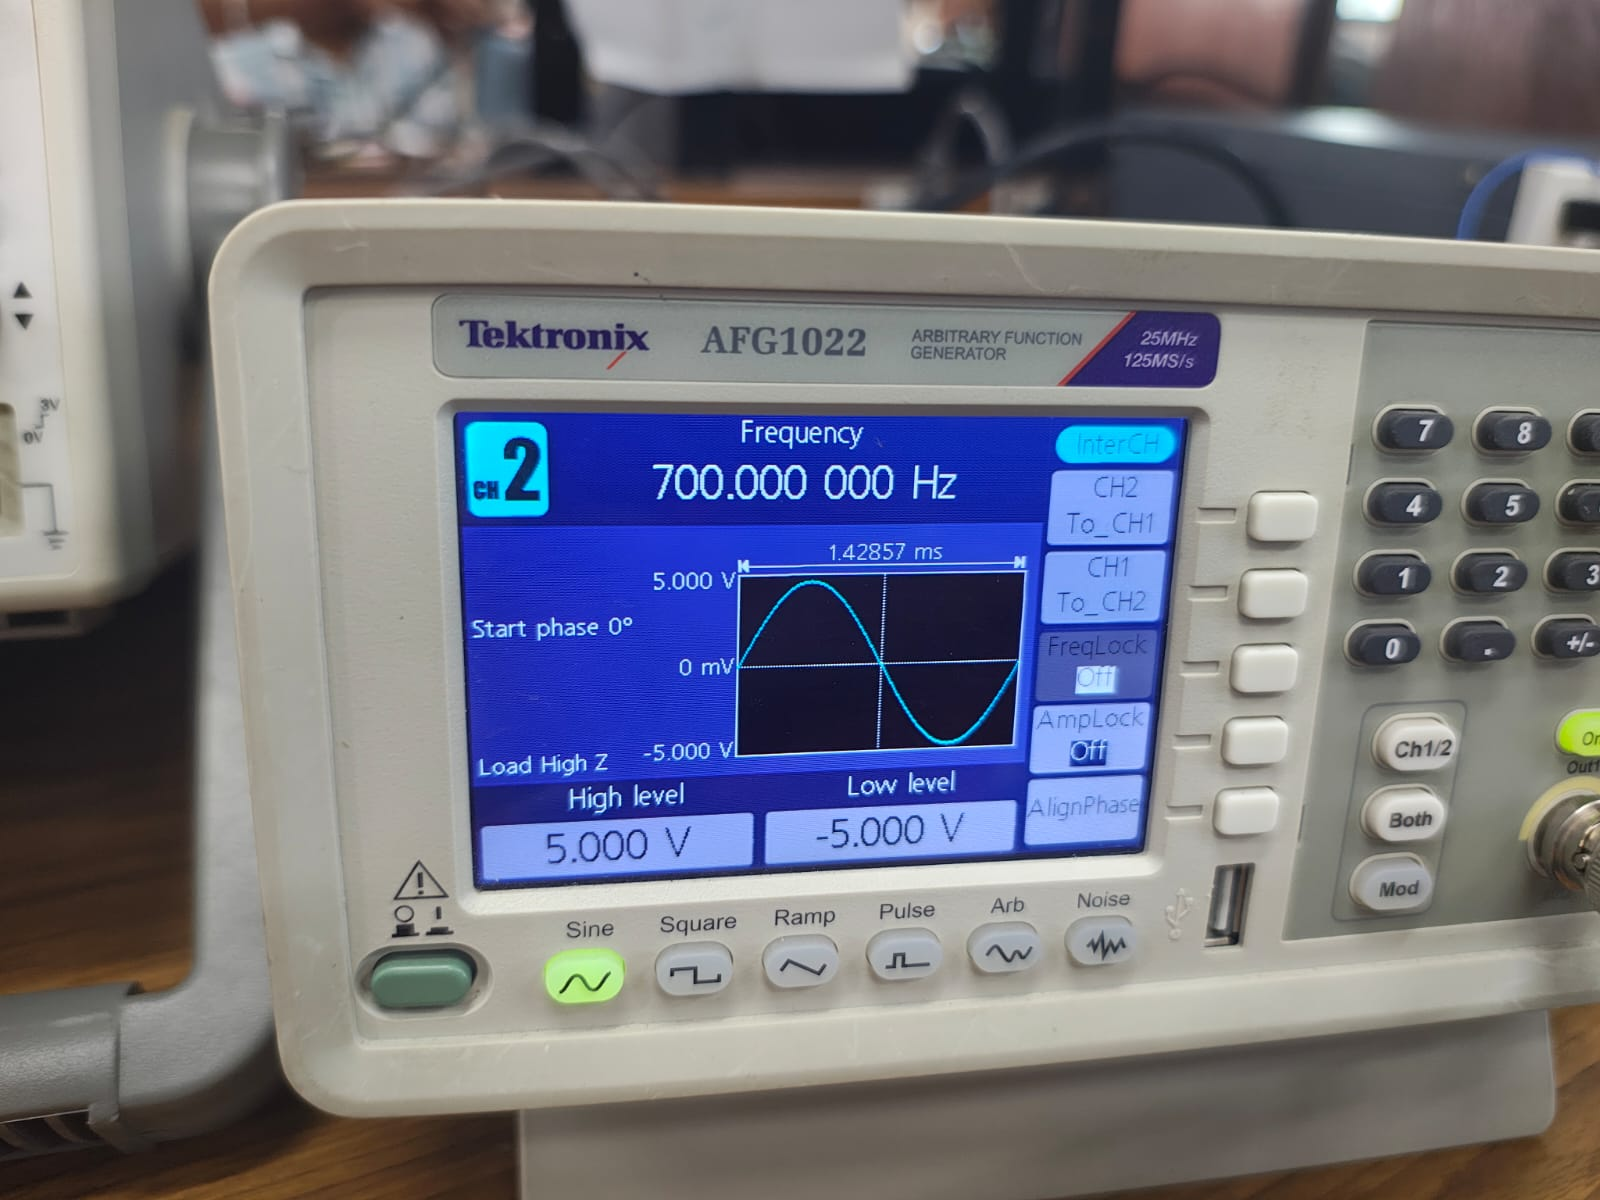
\includegraphics[ width=0.5\textwidth]{./Pictures/Highpass/Highpass12.jpeg}}
\end{figure*}
\FloatBarrier

\begin{figure*}[!htb]
    {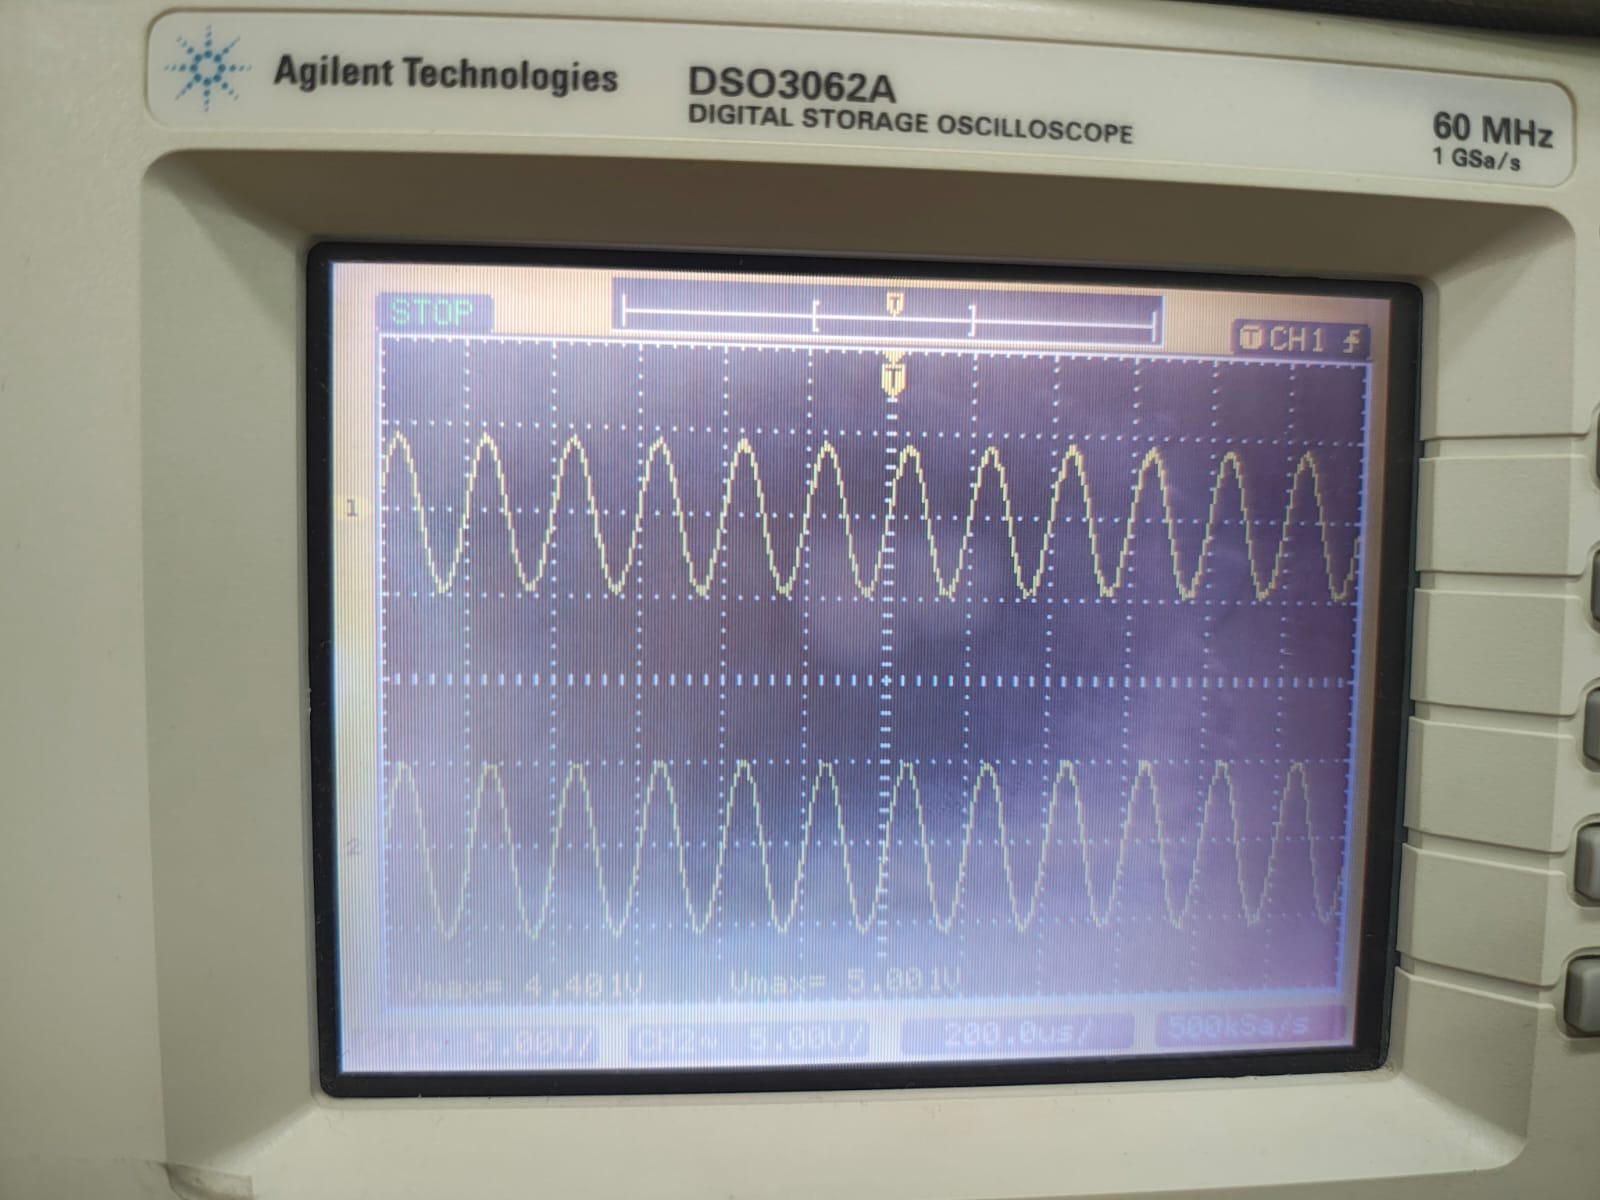
\includegraphics[ width=0.5\textwidth]{./Pictures/Highpass/Highpass19.jpeg}}
    \hspace{\fill}
    {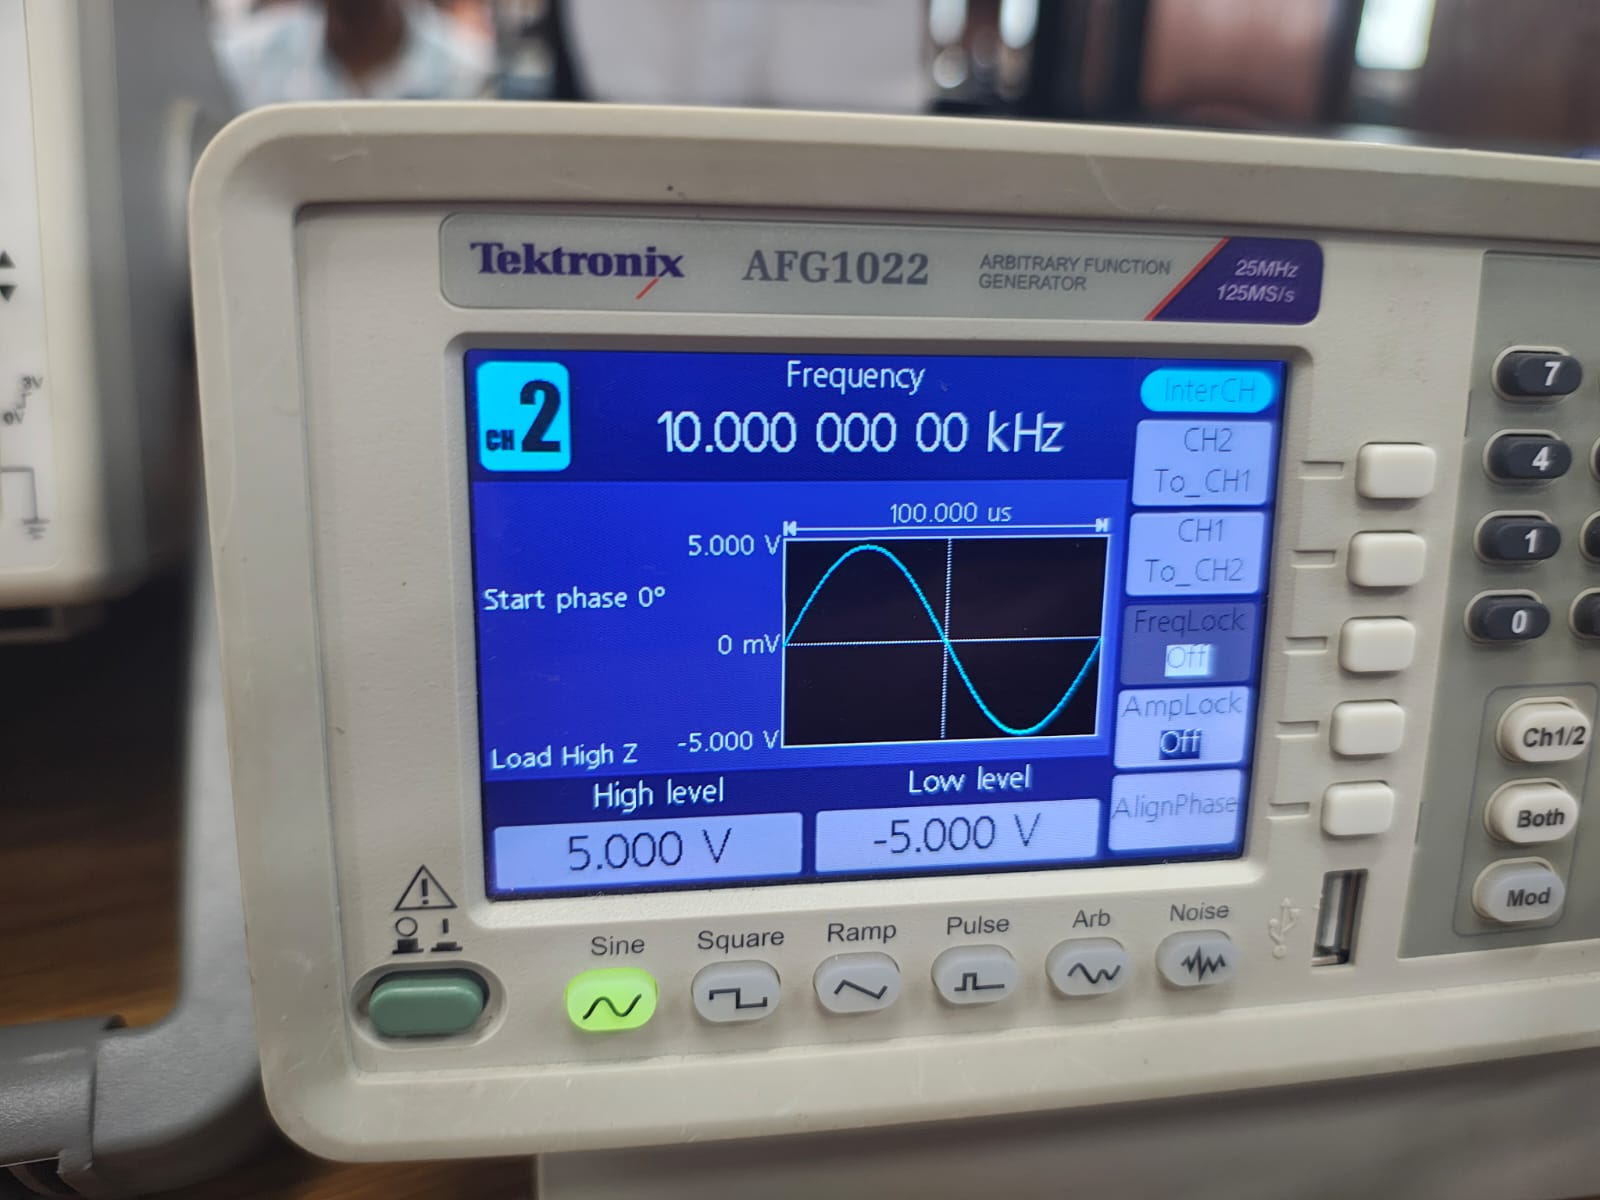
\includegraphics[ width=0.5\textwidth]{./Pictures/Highpass/Highpass20.jpeg}}
\end{figure*}
\FloatBarrier

\subsection{Band-Pass Filter}
Let $R_1, C_1$ be for Low-Pass filter, and $R_2, C_2$ be for High-pass Filter.
\begin{align*}
    R_1 &= 1k\Omega, C_1 = 200nF\\
    R_2 &= 4.7k\Omega, C_2 = 200nF
\end{align*}

\begin{table}[h]
\centering
\begin{tabular}{|c|c|}
\hline
$\log(\omega)$ & $20 \log(|H(s)|)$ \\
\hline
2.4971 & -16.8328 \\
2.6433 & -13.6309 \\
2.7982 & -9.6772 \\
2.9743 & -5.8112 \\
3.0992 & -4.0935 \\
3.1961 & -3.0461 \\
3.4002 & -2.6601 \\
3.4971 & -3.2457 \\
3.5763 & -4.0963 \\
3.7982 & -7.9545 \\
3.9743 & -11.8281 \\
4.0992 & -15.9176 \\
4.2753 & -19.6593 \\
4.4971 & -23.2482 \\
\hline
\end{tabular}
\caption{Logarithmic frequency response data for band-pass filter}
\label{tab:freq_response}
\end{table}
\FloatBarrier

\begin{figure*}[!htb]
    {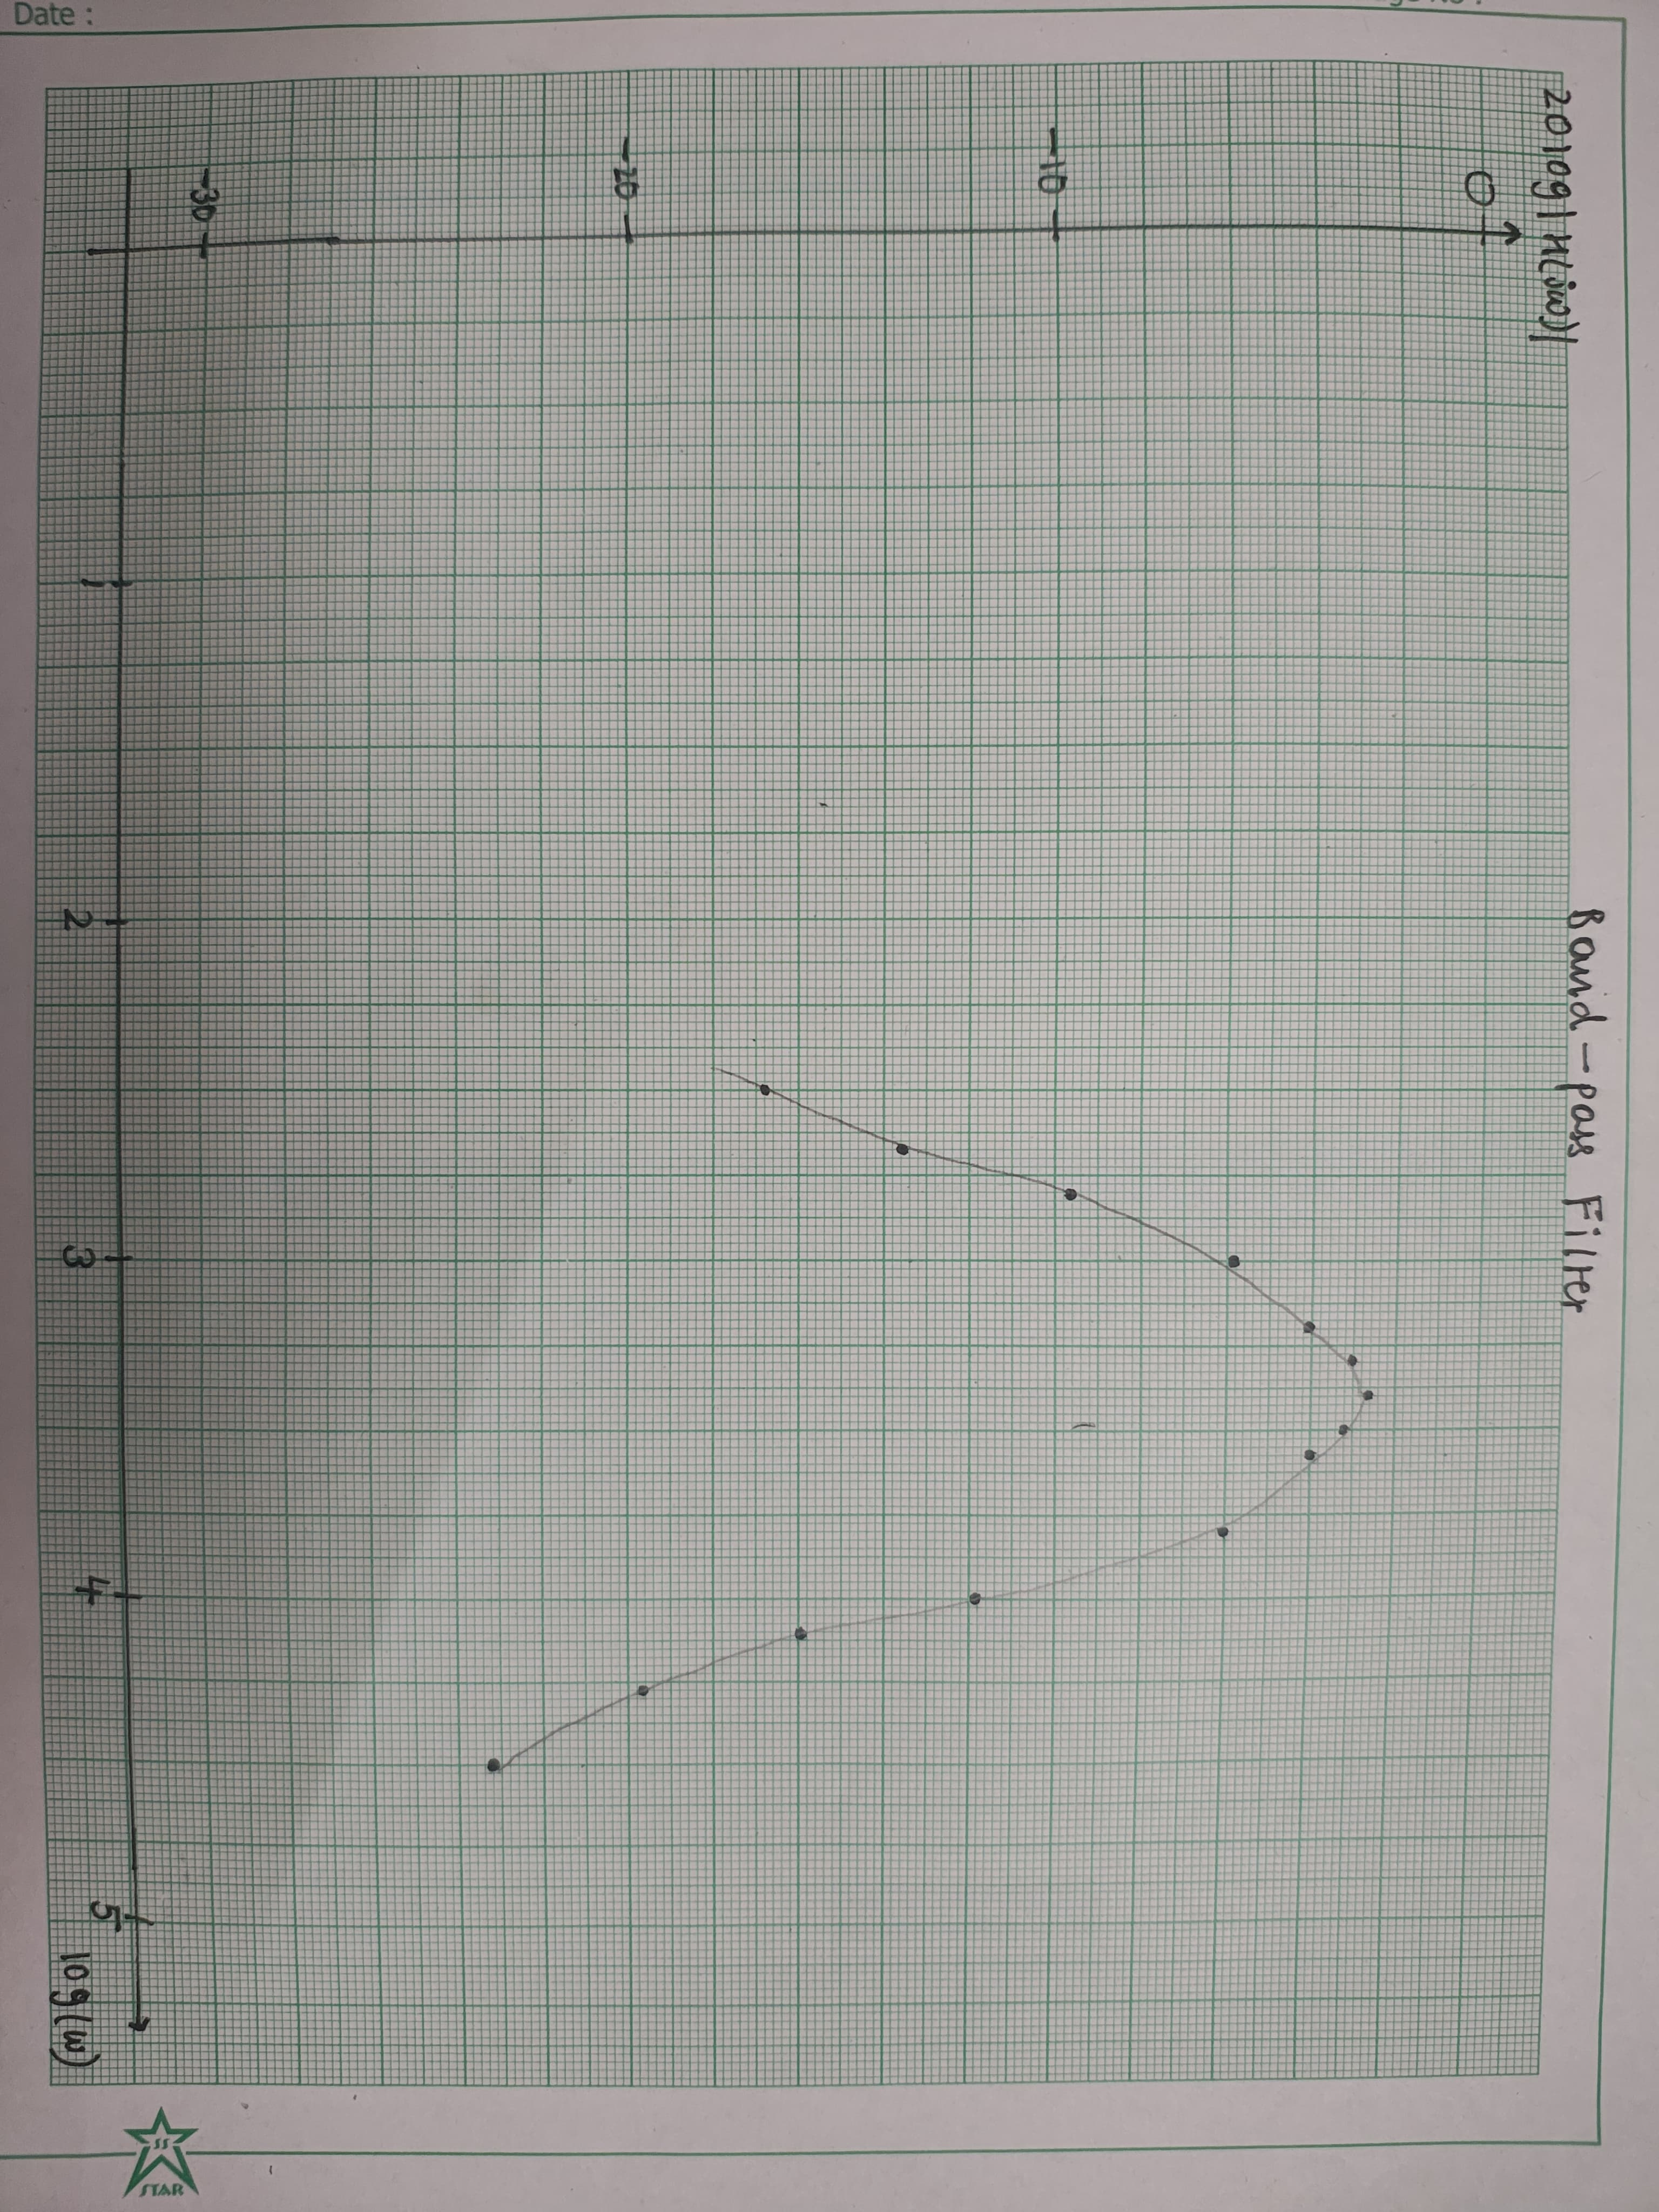
\includegraphics[ width=1\textwidth]{./Pictures/band_pass_bode.jpeg}}
    \caption{Bode Plot for Band-Pass Filter}
\end{figure*}
\FloatBarrier

\begin{figure*}[!htb]
    {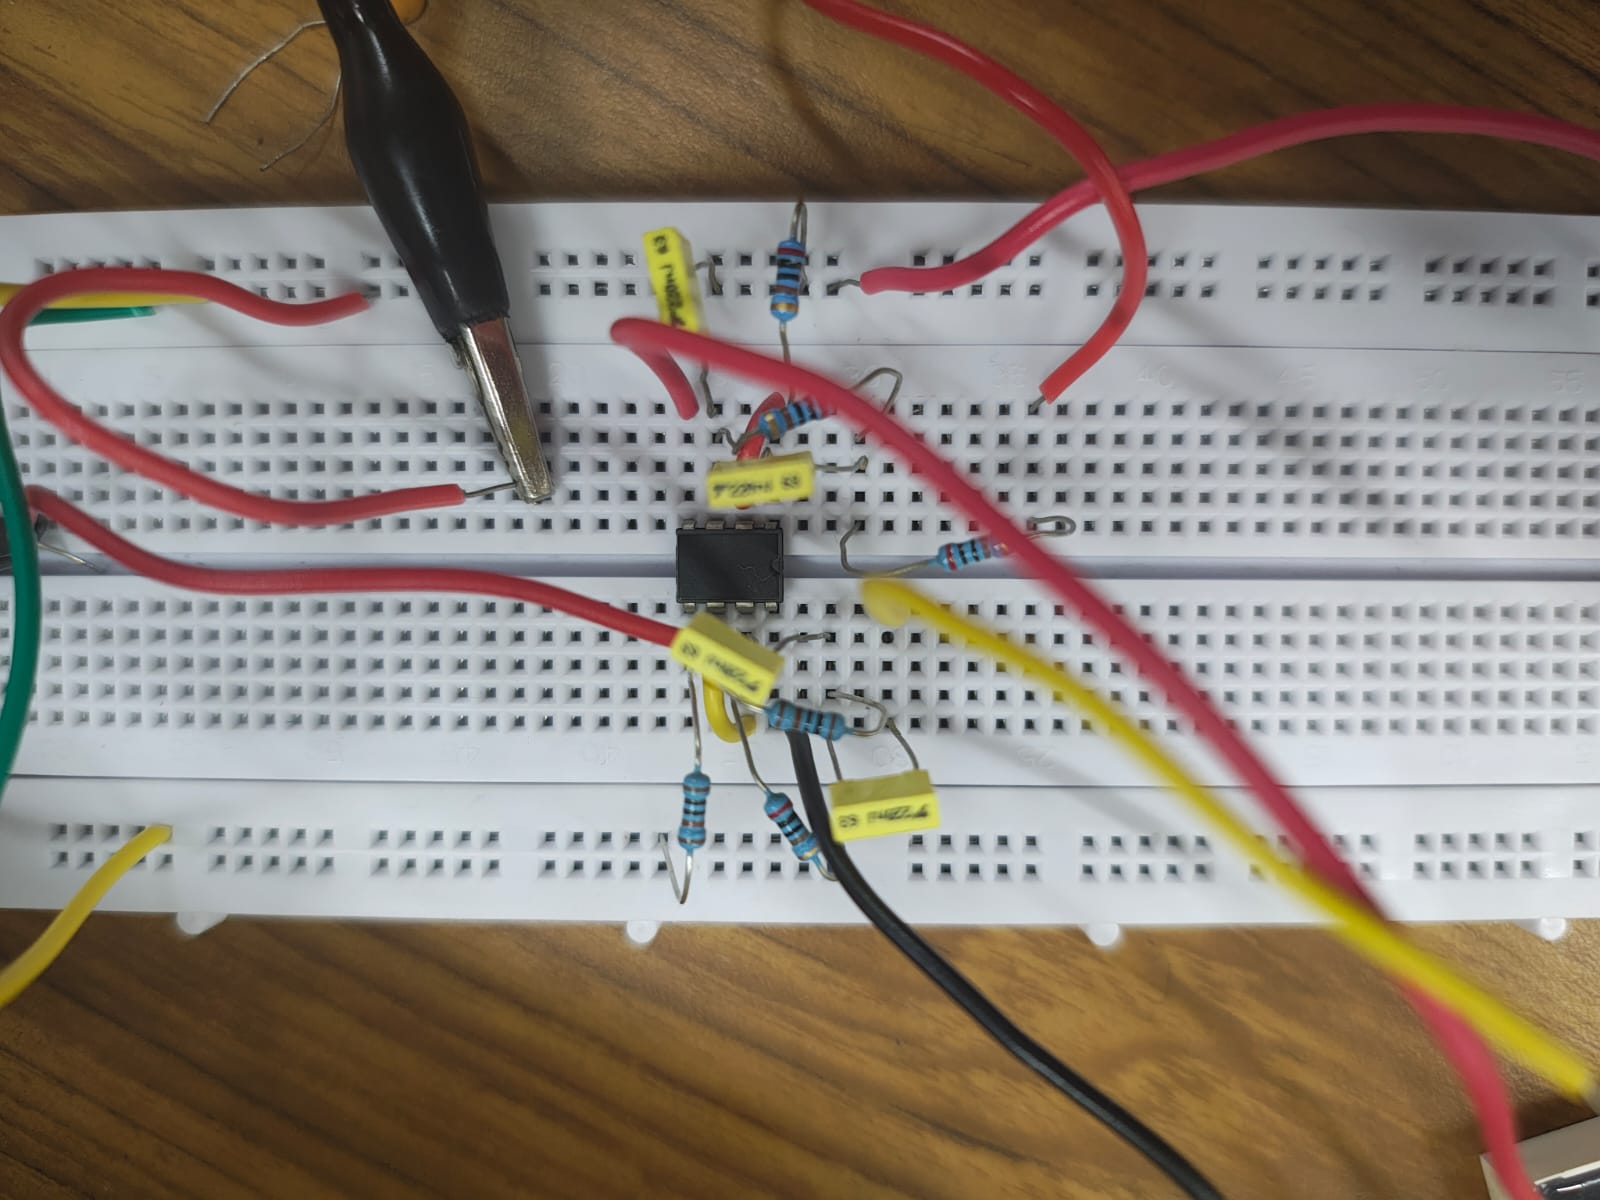
\includegraphics[ width=1\textwidth]{./Pictures/high_pass_circuit.jpeg}}
    \caption{Circuit for Band-Pass Filter}
\end{figure*}
\FloatBarrier

\begin{figure*}[!htb]
    {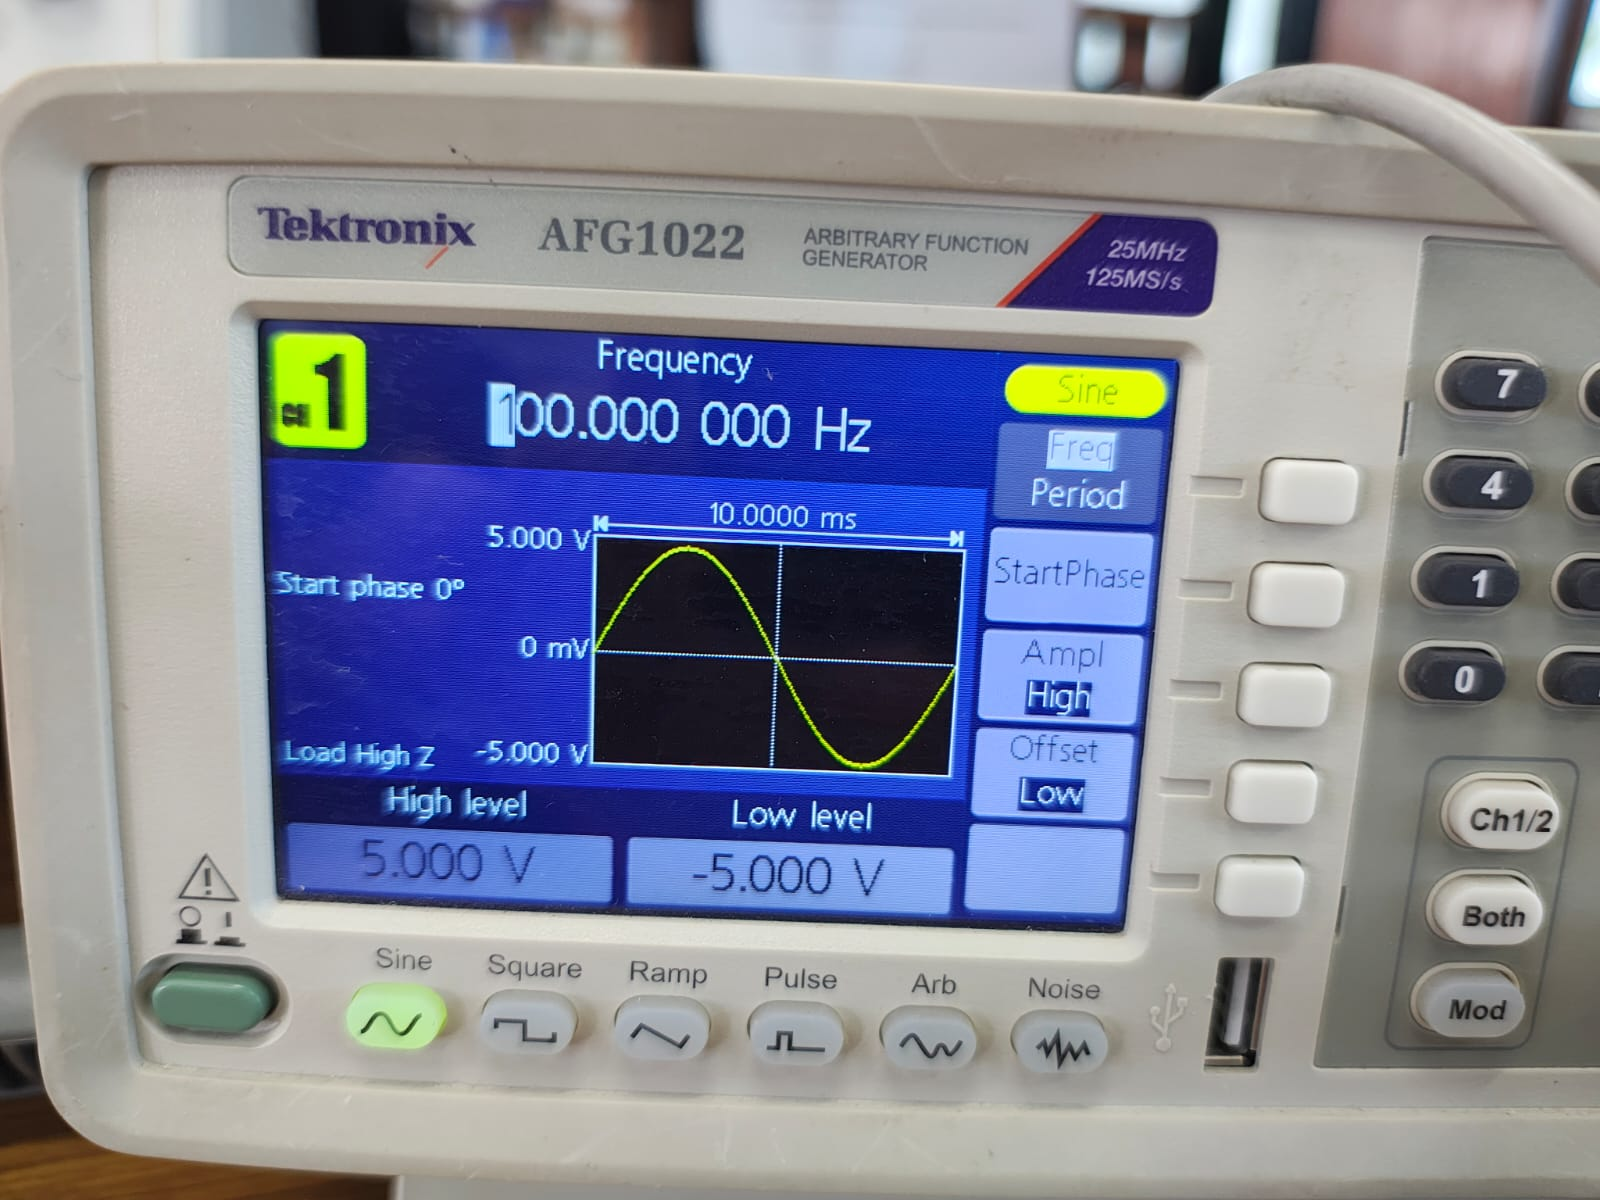
\includegraphics[ width=0.5\textwidth]{./Pictures/Bandpass/Bandpass3.jpeg}}
    \hspace{\fill}
    {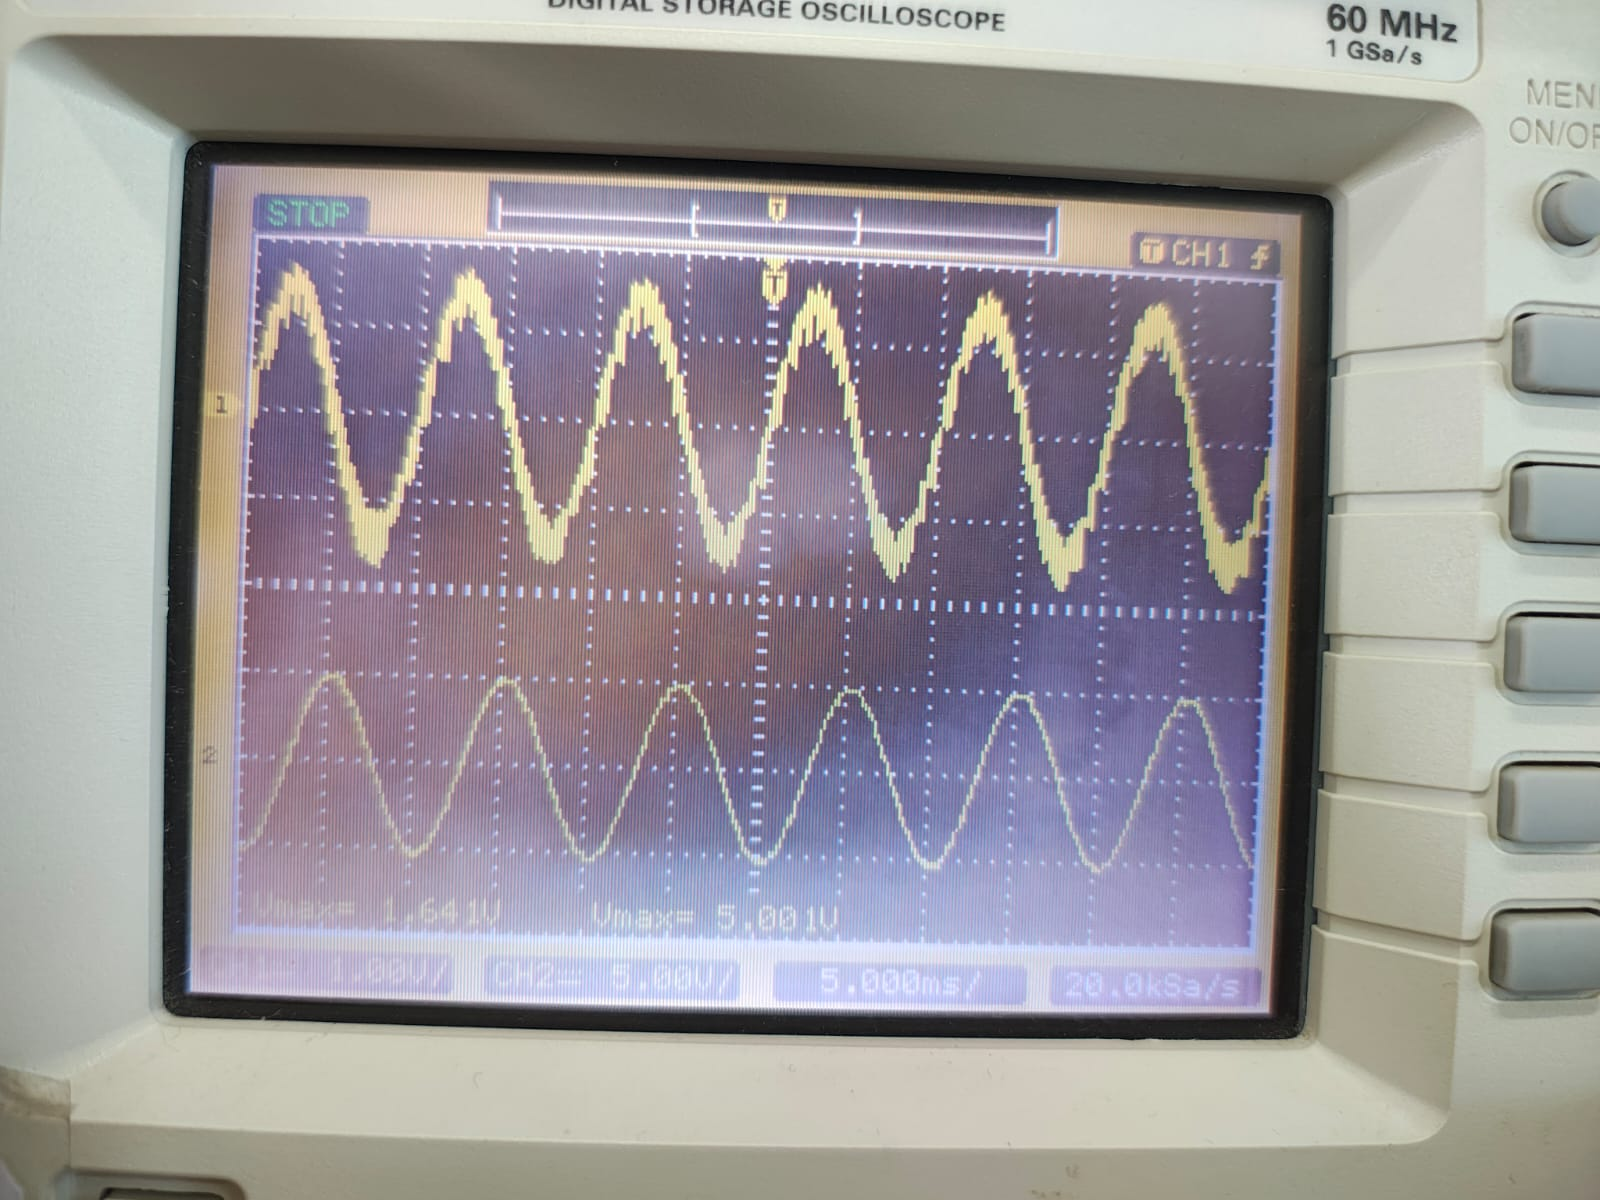
\includegraphics[ width=0.5\textwidth]{./Pictures/Bandpass/Bandpass4.jpeg}}
\end{figure*}
\FloatBarrier

\begin{figure*}[!htb]
    {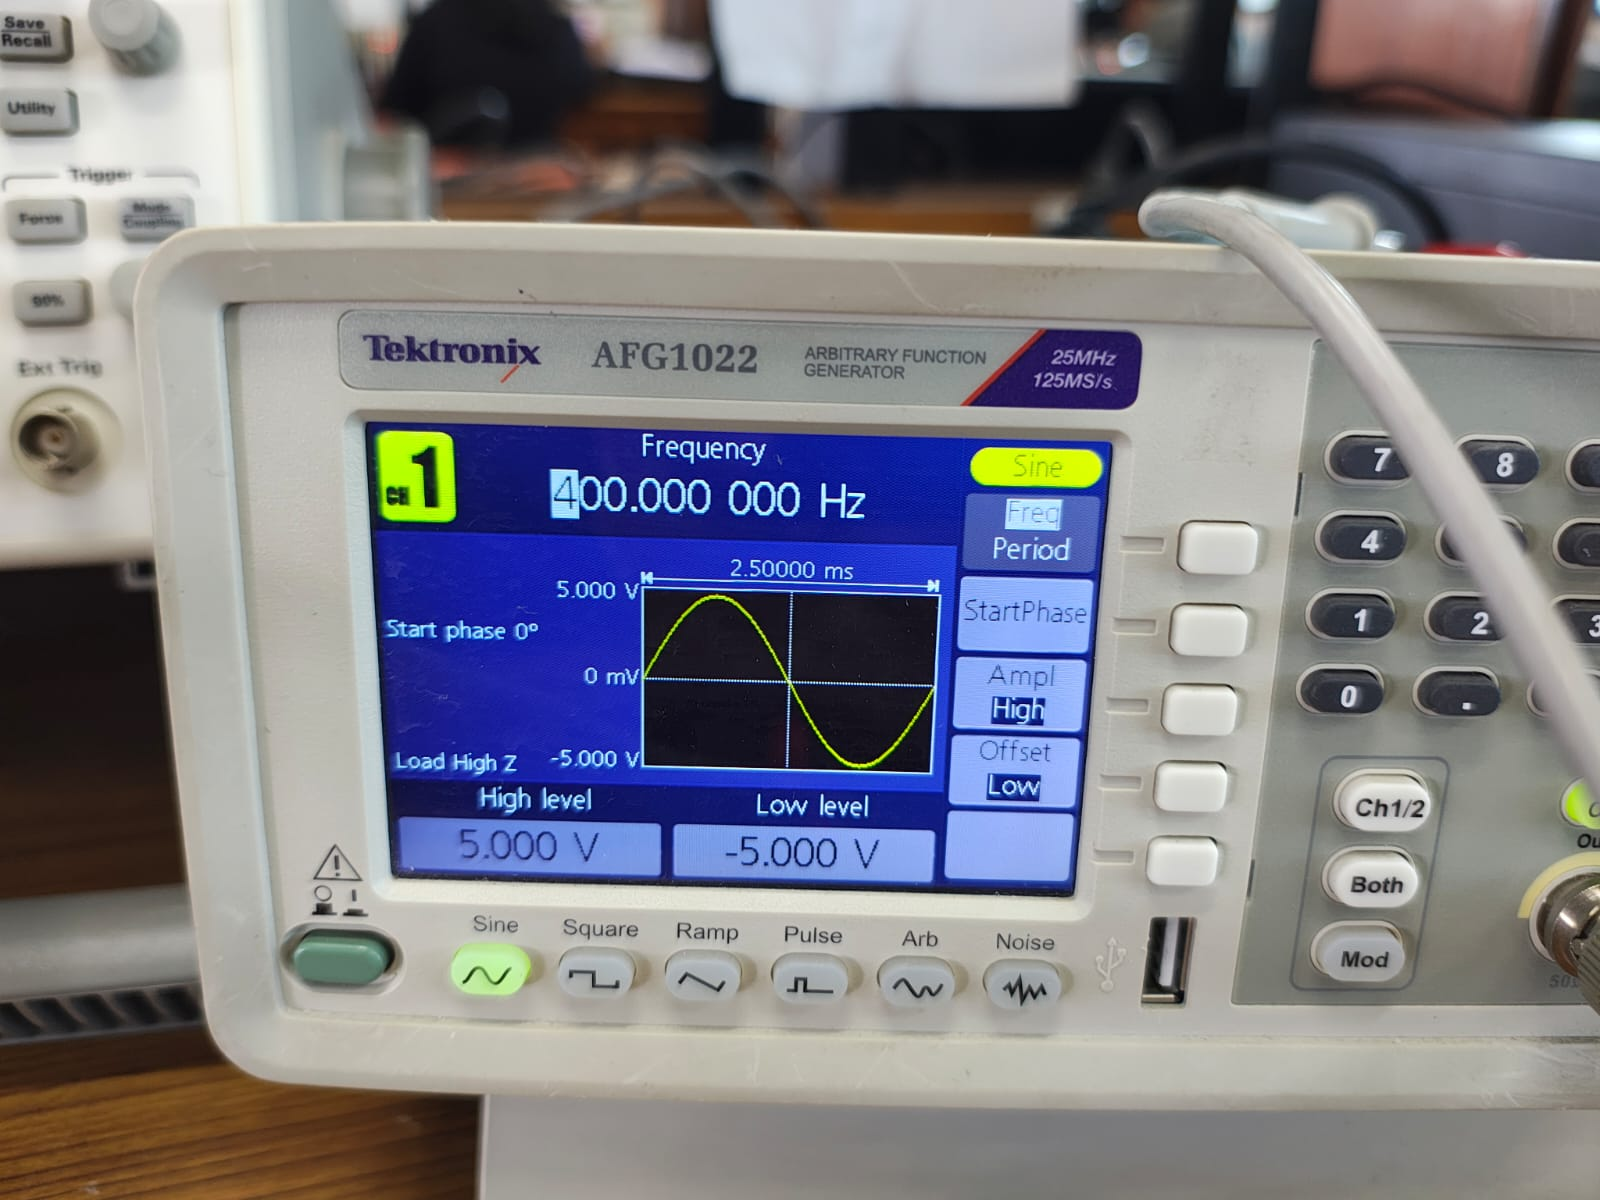
\includegraphics[ width=0.5\textwidth]{./Pictures/Bandpass/Bandpass11.jpeg}}
    \hspace{\fill}
    {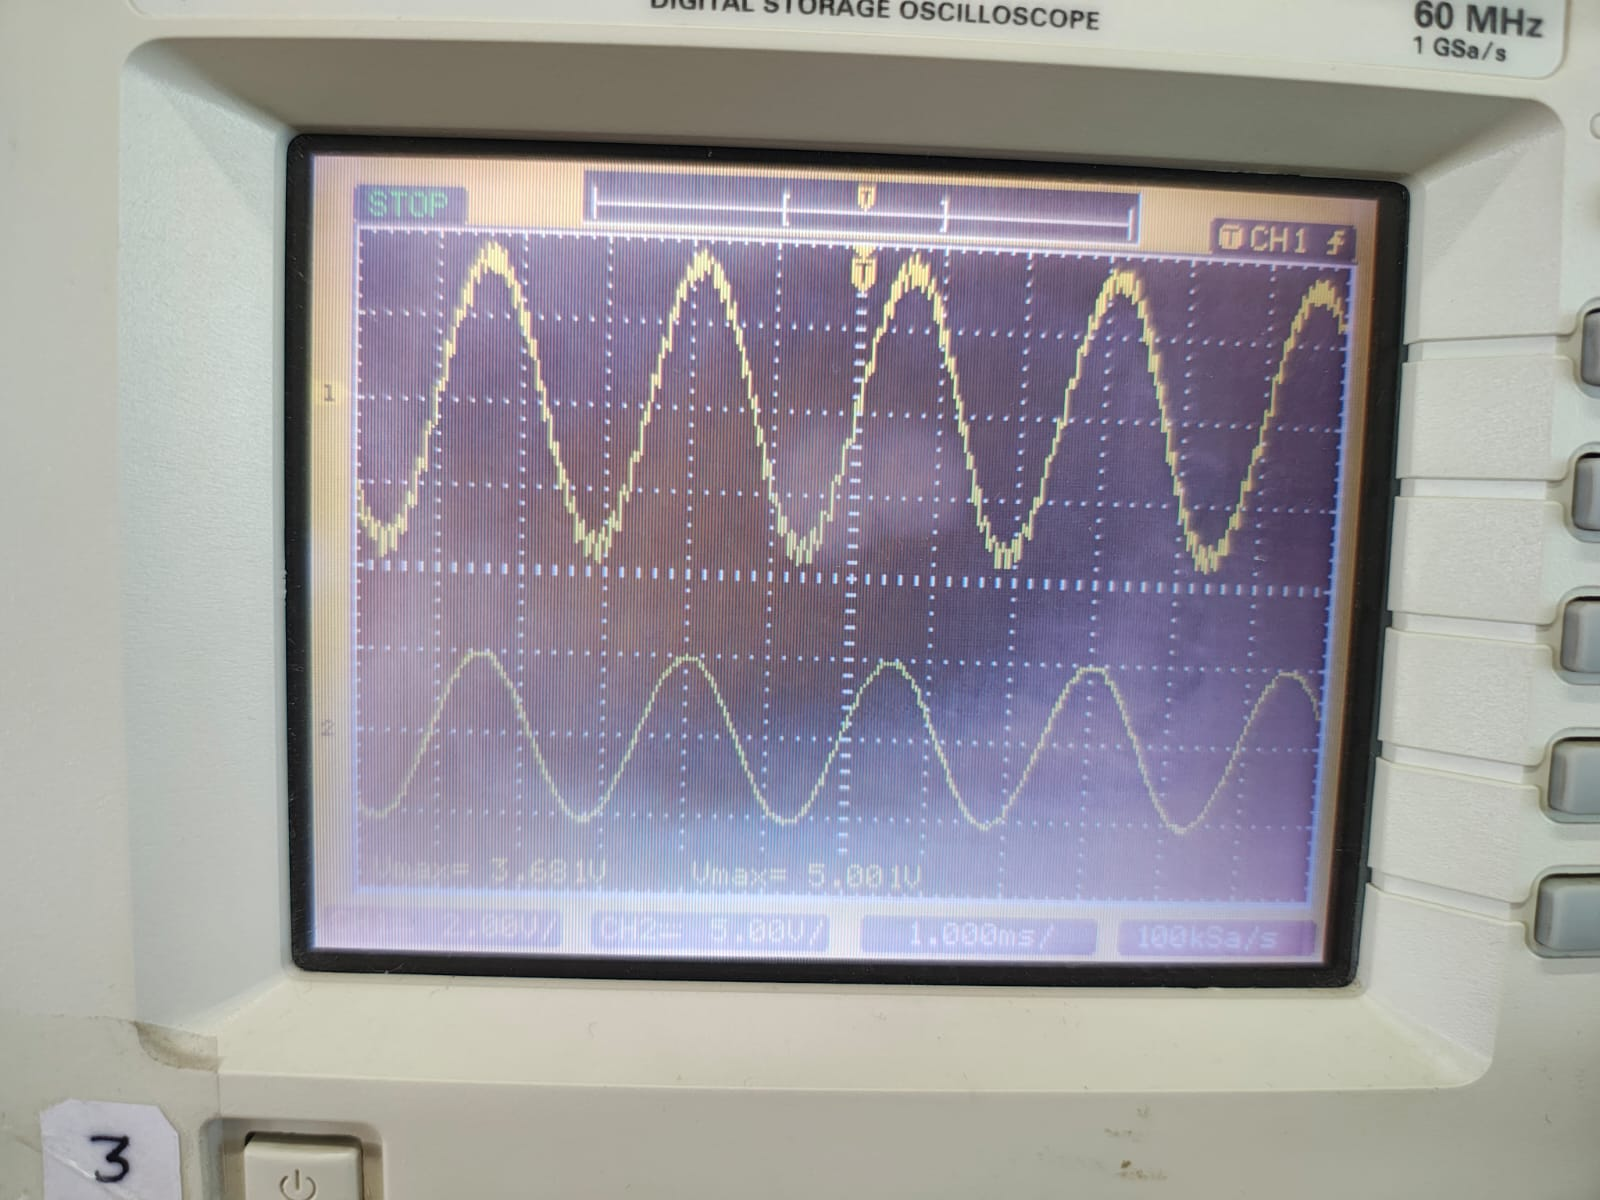
\includegraphics[ width=0.5\textwidth]{./Pictures/Bandpass/Bandpass12.jpeg}}
\end{figure*}
\FloatBarrier

\begin{figure*}[!htb]
    {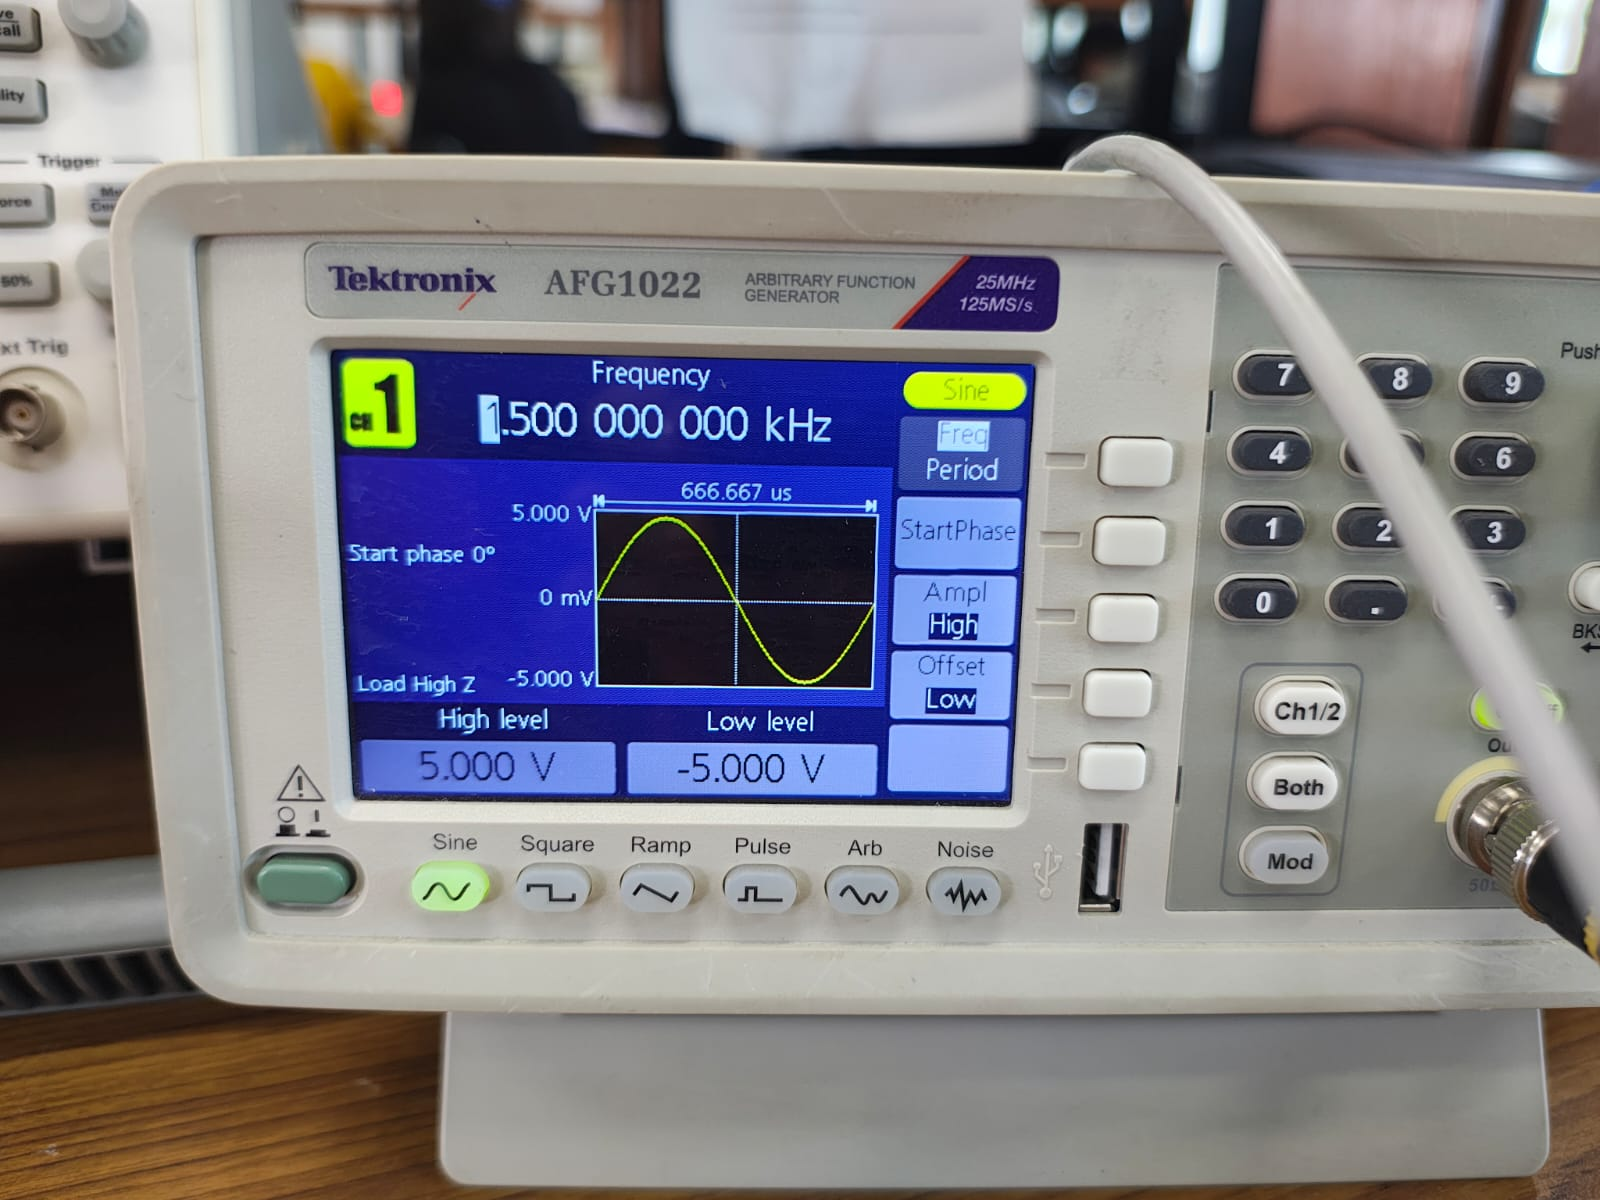
\includegraphics[ width=0.5\textwidth]{./Pictures/Bandpass/Bandpass19.jpeg}}
    \hspace{\fill}
    {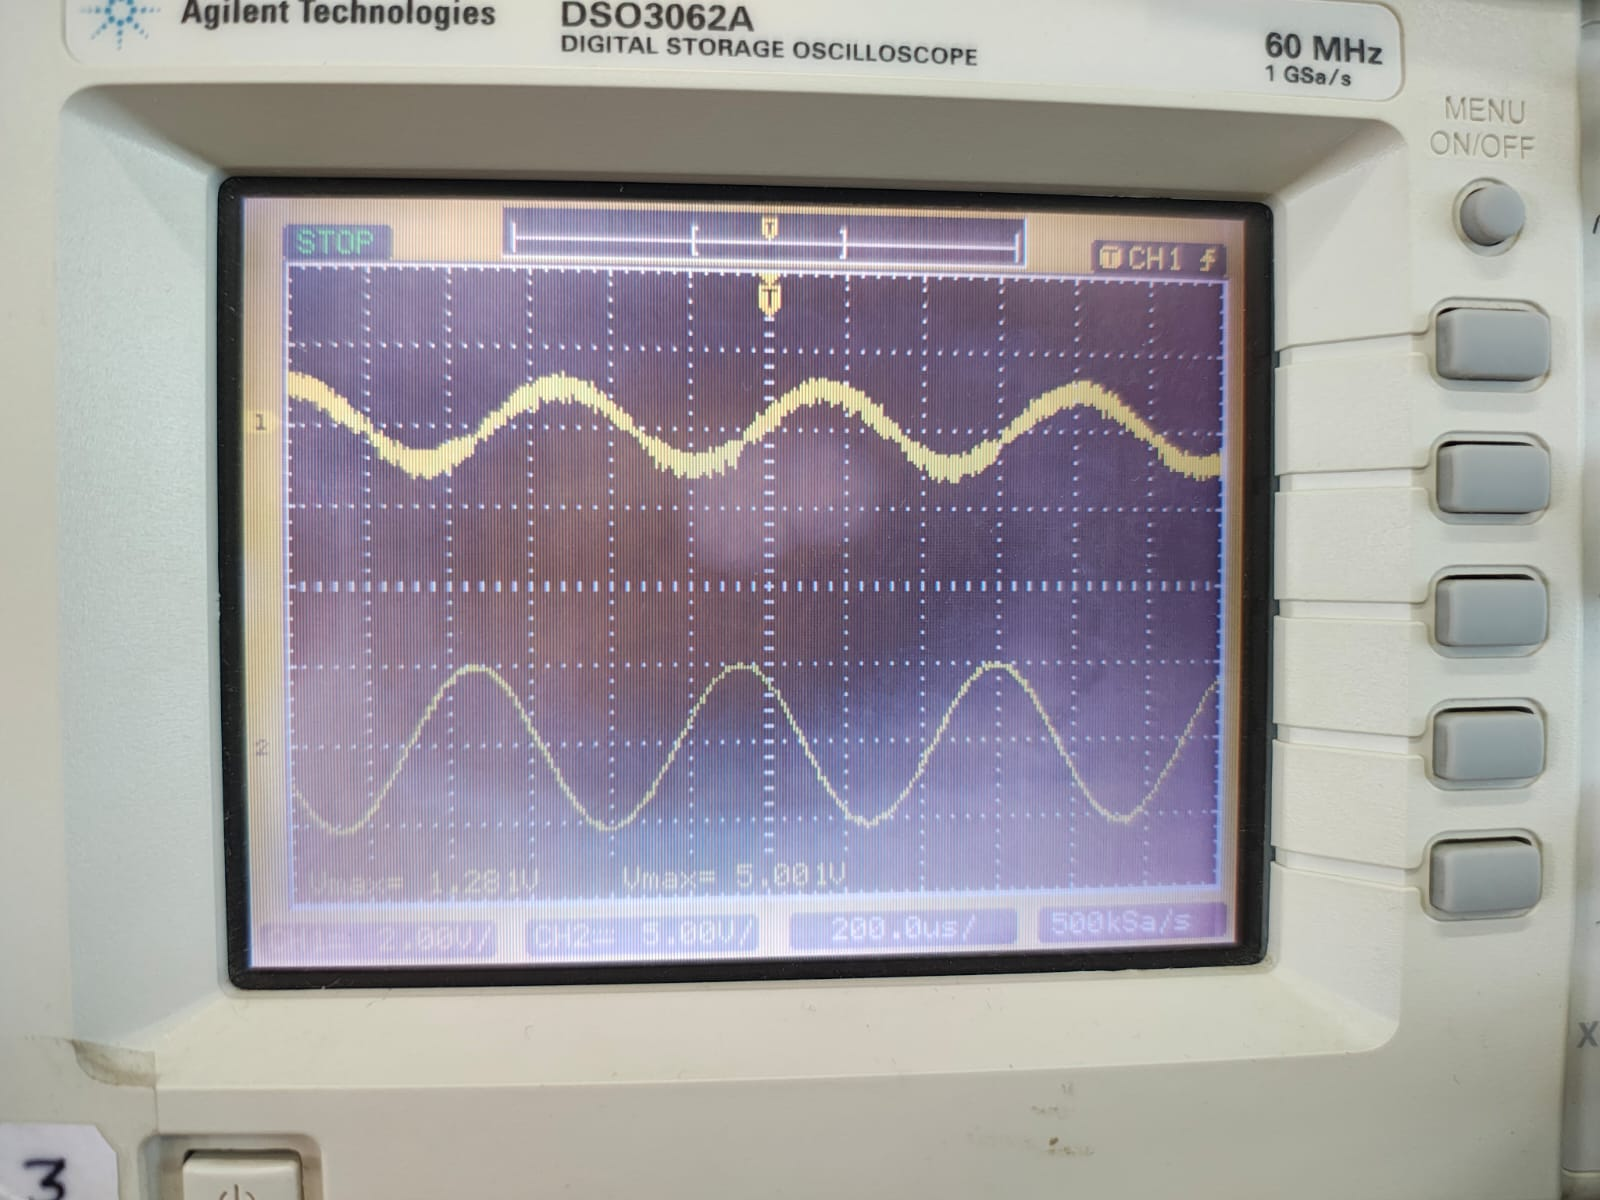
\includegraphics[ width=0.5\textwidth]{./Pictures/Bandpass/Bandpass20.jpeg}}
\end{figure*}
\FloatBarrier

\section{Verification Codes and Pictures}
All the pictures taken are provided below,
\url{https://github.com/AbhimanyuKoushik/EE1200/tree/main/Lab6/Pictures}

Python verification codes are provided below,
\url{https://github.com/AbhimanyuKoushik/EE1200/tree/main/Lab6}

\section{Conclusion}

This experiment successfully demonstrated the design and implementation of a bandpass filter using cascaded Sallen-Key second-order filters.

The Sallen-Key topology proved to be an effective and practical solution for implementing active filters with predictable characteristics. The cascading method for creating a bandpass filter from high-pass and low-pass sections was verified to be a viable approach.

\end{document}
